\documentclass[tcc]{ic}

\hypersetup{
    colorlinks = {true},
    linktocpage = {false},
    plainpages = {false},
    linkcolor = {Blue},
    citecolor = {Blue},
    urlcolor = {Red},
    unicode = {true},
    pdftitle = {Alexis Rapport des enseignements à l'IUT UPPA du 18-09-2023 au 27-10-2023}, 
    pdfauthor = {Alexis Déhu},
    pdfsubject = {Rapport de mes enseignements reçus à l'IUT de Mont-de-Marsan pour la première période de ma deuxième année de BUT R&T du 18-09-2023 au 27-10-2023},
    pdfkeywords = {activités, alternance, iut, but, rt, aditu, uppa, pau, bidart}
}

\usepackage{algorithm}
\usepackage{algpseudocode}
\usepackage[graphicx]{realboxes}
\usepackage{rotating}
\usepackage{lscape}

\makeatletter
\renewcommand{\ALG@name}{Algoritmo}
\renewcommand{\listalgorithmname}{List of \ALG@name s}
\makeatother

\newcolumntype{Y}{>{\centering\arraybackslash}X}

\begin{document}

    % Inclui o preâmbulo do documento (Informações da capa e contracapa)
    \titulo{Rapport des enseignements à l'IUT}

\autor{Alexis Déhu}{adehu@univ-pau.fr}{}


\orientador{M. Angel Abénia}{}{}{}{}
%\examinador{M. Guillaume Devesa}{}{}{}{}

% \examinadorDois{Nome}{}{Instituto de Computação}{Universidade Federal de Alagoas}{Prof. Me.}

\dataMesAno{Octobre}{2023}{}

    \selectlanguage{english}
    
    % Capa, contracapa e avaliadores
    \capa

    % \aprovacao
    
    % Agradecimentos
    % \begin{agradecimentos}

Obrigado

\end{agradecimentos}
    
    % Resumo e Abstract
    \begin{resumo}

    Cette deuxième période la plus longue d'enseignements à l'IUT (5 semaines) nous a permis d'aborder un vaste champ de compétences extrêmement utiles et intéressantes selon moi.
    \\ \\
    Nous avons couvert trois modules de notre parcours cybersécurité orienté vers la sécurisation du service DNS avec DNSsec, de la compréhension des attaques utilisées sur des protocoles répandus dans les réseaux locaux d'entreprises et de la compréhension des technologies et pratiques de chiffrement de nos données.
    \\
    Nous avons aussi aussi à manipuler et intégrer des pare-feux physiques dans un réseau local d'entreprise selon leur besoins.
    \\ \\
    Aspect télécommunications, nous avons abordés les réseaux cellulaires 2G, 3G, 4G et d'autres en profondeur, en parallèle avec l'étude physique et mathématique de moyens transmissions modernes d'émission-réception.
    \\ \\
    Un module intéressant était aussi consacré à l'automatisation de nos tâches d'administrations des systèmes et des réseaux. En complément de l'apprentissage d'un anglais professionnalisé et d'un travail sur notre communication.
    
    \palavrasChave{sécurisation; protocoles; ARP; ICMP; DNS; chiffrement; cryptographie; clés; chiffrement symétrique; chiffrement asymétrique; intégrité des données; confidentialité; authentification; authenticité; signature; certificat; fonctions mathématiques et algorithmiques; OFDM; COFDM; MIMO; CDMA; TDMA; FHSS; féseaux cellulaire; filtres numériques; filtres analogiques}
\end{resumo}
    
    % Sumário
    \renewcommand*\contentsname{Table des matières}
    \tableofcontents
    \thispagestyle{empty}
    
    % Início dos capítulos
    \inicio
    
    \renewcommand{\figurename}{}
\mychapter{R3Cyber16 Méthodologie du pentesting (24h)}{cap:r3c16}
\lhead{R3Cyber16 Méthodologie du pentesting (24h)}

\vspace*{0.2cm}%
      \large
      \href{\@orientadorPagina}{\color{black}Enseignant\\Mr. Jean-Jacques Bascou}\\%
\vspace*{0.5cm}%

Le module R3Cyber16 est le premier module que nous avons eu dédié à la "cybersécurité". Celui-ci abordait les étapes d'un test d'intrusion professionnel lors de ses cours théoriques. Lors des séances de travaux dirigés et pratiques, nous devions comprendre des notions de sécurité d'un SI \textit{système d'information} et leur prévention.
\\ \\
J'aborde en première partie un résumé des enseignements théoriques que j'ai pu avoir lors de ce module. J'interprêtre ensuite ce que nous avons couvert lors des cours dirigiés et des travaux pratiques. J'en conclu par mon impression sur le module et ce que j'en ai à retenir.

\section{Apprentissage théorique des étapes d'un test d'intrusion}

Deux grandes écoles de tests d'intrusion sont prédominantes : la famile OWASP pour le web et les CMS \textit{Content Management System}; \& celle PTEST \textit{Penetration Testing Execution Standard} pour les tests d'intrusion globalisés à un SI ou un groupe de SI.
\\ \\
Dans le cadre de notre formation, nous nous sommes concentrés sur la famille PTEST. Celle-ci définissant un ensemble de normes et de bonnes pratiques, par étapes prédominantes pour un test d'intrusion sur un SI de manière professionnelle.
\\ \\
Un test d'intrusion est caractérisé par un ensemble de processus, qui doivent prouver ou non la sécurité tout ou partie d'un SI, dans des conditions réelles.
\\ \\
Selon le contexte d'intrusion définit au préalable, nous pouvons catégoriser trois types de tests : les tests sous boîtes noires avec aucune connaissance de l'environnement, les tests à boite grise en ayant en partie connaissance de la structure dans laquelle l'attaquant va évoluer et ceux à boîtes blanches avec une connaissance totale de l'environnement.
\\ \\
Chacune de ces familles respectent un ensemble de règles à respecter selon le besoin du test d'intrusion et la criticité du système touché. Ainsi, le PTEST comporte sept grandes étapes que chaque testeur d'intrusion en entreprise se doit de respecter.
\\ \\
La \textbf{période de pré-engagement} définit le périmètre de l'étude (équipements, logiciels, personnels...), avec une date \& une horaire pour l'activité, un contexte global (depuis l'extérieur, l'intérieur...), le niveau de connaissance que doit avoir l'attaquant (vu boîtes - noire l'attaquant ne connaît rien), la limite de son étude (pas les serveurs de sauvegarde) et ses mandats d'autorisation ou des propositions commerciales.
\\ \\
Une fois que l'attaquant a son champs d'action, il doit approfondir sa connaissance du milieu : il doit s'imprégner d'un maximum d'informations extérieures sur sa cible. Cette \textbf{période de reconnaissance} consiste à obtenir le plus d'informations possibles sur le périmètre de son étude (équipements, systèmes d'exploitation, personnel l'utilisant...) par mails bien agencés, analyse systèmes exposés à internet... Ce cadre est encore une fois définit par les boites : blanches - on nous donne tout, grise - on nous donne des informations souvent pour gagner du temps, que l'étude ne revienne moins chère \& noires tout est à faire (HUMINT \textit{Human Intelligence}, OSINT \textit{Open Source Intelligence}...).
\\ \\
Par la suite, après son étude globalisée de la structure, celui-ci va établir une \textbf{modélisation de la menace} \textit{threat modeling}. Cette étape se traduit par une analyse des risques associés à l'activité entreprise en terme de sécurité (accès aux mails, communication entre sites...). Ce qui en résulte en l'étude de la probabilité qu'une menace exploite une vulnérabilité trouvée. Il effectue donc une hiérarchisation du niveau de criticité des services qu'il va toucher, en acceptant les conséquences d'un risque, leur déplacement ou leur limitation (en rapport avec ce qu'il a vu étape de reconnaissance).
\\ \\
La quatrième étape d'\textbf{analyse de vulnérabilité} consiste à rechercher des vulnérabilités exploitables sur une ou plusieurs cibles, plus ou moins critiques sur le threat model. Ces deux étapes peuvent dans certains cas être inversées. L'attaquant va rechercher des vulnérabilités à exploiter sur les SI par différents moyens : reverse-engineering, outils d'OSINT, d'HUMINT, scripts... Il peut s'aider du répertoire de vulnérabilités CVE \textit{Common Vulnerabilty and Exposures} répertoriant les vulnérabilités majeures des services connus et celui de leur criticité CVSS \textit{Common Vulnerability Scoring System} pour indiquer leur niveau de criticité de 1 à 10.
\\ \\
Une fois des vulnérabilités trouvées ou non, l'attaquant va essayer de les exploiter pour arriver à ces fin : \textbf{étape d'exploitation}. Des procédures simples de démonstration d'exploitation de vulnérabilités \textit{proof of concept} existent et sont souvent utilisées. L'attaquant peut aussi exploiter une faille trouvée manuellement, automatiquement par des outils déjà créées, ou concevoir ses propres outils étudiés pour l'exploitation d'une vulnérabilité non répertoriée, trouvée sur le tas \textit{zero day}.
\\ \\
Une fois l'exploitation d'une vulnérabilité réalisée sur un SI, l'attaquant va pouvoir changer son contexte d'attaque en essayant de trouver d'autres machines exploitables depuis la nouvelle machine infectée. Un deuxième objectif est de souvent s'installer de manière pérennisée. Cette étape de \textbf{post-exploitation} se constitue généralement d'une élévation de privilèges sur la machines si besoin, une attaque latérale à d'autres machines ou d'un changement de réseau pour un nouveau découvert sur la machine compromise. Pour ce dernier exemple, il est parfois nécessaire de revenir à l'étape de reconnaissance.
\\ \\
La dernière étape des sept étant le \textbf{rapport} ou le \textit{reporting} des tentatives - les points positifs et négatifs. Elle s'en suit généralement d'une proposition d'amélioration de la sécurité globale du SI pour amener la discussion vers la conclusion sur les risques qui lui ont été demandés de prouver. L'étude essayant de prouver que ceux-ci sont moindres car suffisamment protégés, à les déplacer, ou de les laisser car acceptable. Un attaquant n'ayant pas trouvé de faille sur un SI ne veut pas dire que le SI est bien sécurisé, tout dépend de l'approche / la méthodologie que l'attaquant aborde. Ce n'est que grâce au rapport que vous pourrez conclure que la sécurité de votre SI correspond à vos attentes.

\section{Application et découverte de l'analyse de sécurité}

Lors des travaux pratiques et dirigés de ce module, nous avons été guidé dans la manipulation d'outils pour appliquer succinctement les étapes du modèle PTEST. L'objectif à terme étant de savoir les mettre en lien afin de réaliser un véritable test de pénétration.
\\ \\
Une première partie était dédiée à l'étude de l'étape de reconnaissance. Celle-ci nous montrant des méthodologies applicables via l'OSINT, passant par la recherche d'informations sur le réseau cible depuis internet, allant au regard des enregistrements DNS, ou encore par la récupération automatisée des adresses mails présentes sur le site publique cible...  
\\ \\
Rechercher des informations libres d'accès sur la cible permet d'avoir un point de vue global de la structure, autant informatique qu'humain, pour débuter un plan d'analyse par la suite. Le but étant de réunir un maximum d'informations intéréssantes. Tout ce qui est exposé à internet peut être potentiellement compromis ou être utilisé pour une compromission, même une information mineure.
\\
\textit{dig, whois, dnsrecon, dnsenum, nmap, Spiderfoot, The Harvester, dirb utilisés}
\\ \\
La deuxième étape de recherche de vulnérabilités a aussi était couverte par l'analyse plus approfondie du réseau (analyse de ports aggressif, test utilisation protocole SNMP, Openvas pour les scans de SI \& permet de faire remonter un rapport de vulnérabilités)... Cette partie étant l'une des plus techniques, nécessitant une bonne source de connaissance en informatique et en réseau dans un lapse de temps relativement cours. Elle nécessite aussi énormément de savoir manipuler ses outils, une courbe d'apprentissage plus ou moins abbrute peut être ressentie.
\\
\textit{netdiscover, nmap, snmp-check, Openvas, Greenbone utilisés}
\\ \\
Nous avons vu transversalement les attaques par force brute \textit{bruteforce} et par dictionnaire. Cas d'exemple - certains utilisateurs peuvent utiliser le nom de leur animal, de leur enfant, avec une suite de nombre correspondant à une date symbolique, comme un mariage ou une naissance, pour définir leur mot de passe. Avec les informations récupérées sur les personnes et sur l'infrastructure informatique lors de l'étape de reconnaissance, et en connaissance que la cible n'est pas un utilisateur avancé d'informatique : nous pouvons essayer de générer une suite de mot de passe contenant les informations de la victime réagencées pour essayer de trouver son mot de passe sur une machine (Milou235182, Pipou!12/24...).
\\ \\
Cette méthode ayant une limite : le nombre de tentative est très souvent limité. Plus loin que d'essayer de trouver un mot de passe, nous pouvons essayer de comparer la signature du mot de passe (car il est forcément stocké) à cette liste. Les mots de passe ne sont généralement pas enregistrés en clair - si quelqu'un ouvrait le fichier contenant votre mot de passe, il ne pourrait pas le lire. À la place, ceux-ci sont renseignés par empreinte - fonctions mathématiques complexes ne permettant pas de retrouver la source. Des listes d'empreintes sont générées par algorithme de chiffrement, si l'attaquant réussi à récupérer l'empreinte d'un mot de passe \textit{hash} (car stocké quelque part) : il peut le comparer chez lui à une liste de hashs \textit{rainbow list} de mots de passe connus pour essayer de le retrouver, pour peu que votre mot de passe soit courant. Il est aussi possible de "cracker" un mot de passe, mais demandant une force de calcul impressionnante, déjà que la comparaison en demandant beaucoup.
\\
\textit{Crunch, Cewl \& Hydra pour génération de dictionnaire, Hashcat \& John the ripper pour comparaisons}
\\ \\
La dernière étape étudiée fut celle de l'exploitation de vulnérabilités, majoritairement avec Metasploit. Metasploit est un outil permettant de regrouper des exploitations de vulnérabilités connues, c'est une grande boite à outils, un framework... Un bon attaquant, par ses connaissances, devra parfois créer ses propres outils pour ses tests d'intrusion, car utilisation trop spécifique.
\\ \\
Le cheminement d'utilisation de Metasploit se résumé à : rechercher une vulnérabilité (numéro de version d'un logiciel, protocole non sécurisé...), selectionner un \textit{exploit} - un programme dans Metasploit renseigné pour exploiter cette vulénrabilité, et changer son payload (contenu du programme qui est malveillant) pour le remplacer par les informations nécessaires - peuvant être le changement d'une adresse IP, certains paramètres...
\\ \\
L'utilisation de Metasploit est extrèmement intéressante pour beaucoup de cas d'usages, mais il faut tout de même avoir une bonne base théorique des protocoles étudiés pour les appliqués. Aussi avoir de bonnes notions en réseau pour les utiliser correctement. Nous sommes aussi limités par ce qui est présent dans Metasploit, sa courbe d'apprentissage est aussi extrêmement très rapide car simple mais vite limitée par ce qu'il propose, plutôt que de nous faire une collection de nos propres outils pour exploiter les vulnérabilités qu'on trouve.
\\
\textit{montage d'un reverse shell php, utilisation exploit ssh version 1, exploitation/proof of concept log4j par renseignement cve, scan réseau avec Metasploit par arp sweep, élévation de privilège, évasion de conteneur (docker escape), msfvenom, lancement d'un reverse shell par crontab}

\section{Aboutissants de l'enseignement}

Ce module nous a permis de comprendre la méthodologie d'un test d'intrusion professionnel. Nous avons vu un exemple d'application des étapes de l'école PTEST, par l'accompagnement dans l'utilisation d'outils dédiés. Reste à nous de définir nos propres méthodologies, de reprendre, ou s'inspirer de celles vues en cours.
\\ \\
Je retiens que pour un test d'intrusion, une grande connaissance théorique est nécessaire pour espérer en faire un bon : notamment pour rendre un rapport cohérent... Il ne suffit pas de copier-coller des démonstrations d'outils trouvés sur internet, ou encore d'ouvrir Metasploit et espérer faire fonctionner le bon exploit... Apprendre en même temps de découvrir ce qu'on a sous les yeux est possible mais dangereux...
    \renewcommand{\figurename}{}
\mychapter{R3Rom16 Ingénierie de la téléphonie sur IP (1h30)}{cap:r3r16}
\lhead{R3Rom16 Ingénierie de la téléphonie sur IP (1h30)}

\vspace*{0.2cm}%
      \large
      \href{\@orientadorPagina}{\color{black}Enseignant\\Mr. Angel Abénia}\\%
      \normalsize
\vspace*{0.5cm}%

L'enseignement de ce module s'est fait durant la deuxième période d'enseignement à l'IUT. Les 1h30 de cours dispensés sur la première période ont permis de cerner le sujet abordé et de reprendre les bases nécessaires à sa compréhension pour notre retour.
\\ \\
Je me permets uniquement de mentionner ce premier cours dans la première période que l'on a eu à l'IUT pour ces 1h30. Nous y avions revu de la VoIP \textit{Voice over IP} et abordé différenciation avec la ToIP \textit{Telephony over IP}.
    \renewcommand{\figurename}{}
\mychapter{R301 Réseaux de campus (30h)}{cap:r301}
\lhead{R301 Réseaux de campus (30h)}

\vspace*{0.2cm}%
      \large
      \href{\@orientadorPagina}{\color{black}Enseignant\\Mr. Shidoush Siami}\\%
\vspace*{0.5cm}%

Le module R301 avait pour objectif de nous faire manipuler les technologies utilisées dans les réseaux de campus. Sont définis des réseaux de campus de grandes infrastructures informatiques d'entreprise, généralement multi-sites ou complexes. Ainsi, les technologies abordées touchent aux domaines de l'automatisation de tâches - pour prévenir la répétition d'activités manuelles sur un grand nombre de postes -, la gestion de SI à distance - éviter les déplacements fréquents \& favoriser la gestion dynamique d'un réseau -, des tables de routage dynamique, et la redondance de routeur de façade.
\\ \\
Nous avons plus spécifiquement vu dans ce module un renforcement de l'utilisation du protocole SSH \textit{Secure Shell} par l'utilisation de clés asymétriques, le déploiement d'actions simple par SSH avec Ansible, une introduction au routage inter-VLAN, et enfin une utilisation des protocoles OSPF, HSRP, EIGRP \& BGP.

\section{Hardening du protocole SSH}

Nous avons utilisé le protocole SSH par le passé à l'IUT sans l'avoir étudié. Cette fois-ci, nous l'avons étudié et fait du hardening \textit{renforcement} en intégrant l'utilisation de clés plutôt que de mots de passe pour l'initiation d'une session.
\\ \\
Au lieu d'utiliser des mots de passe comme méthode d'authentification, le protocole SSH permet d'utiliser un couple de clé publique \& privée pour s'authentifier. Les clés étant plus robustes au déchiffrement par leur longueur plus importante et aléatoire (1024 bits, 2048...). L'utilisateur peut aussi ne pas connaître le mot de passe de sa session Shell, pour lui restreindre dans ses activités, pas sa connexion.
\\ \\
Les premières séances de travaux pratiques étaient dédiés à la création et l'utilisation des clés sur des machines GNU/Linux. J'ai rajouté une partie pour les intégrer à des équipements Cisco, non présent sur le cours de base, rajouté par la suite. Accessible sur \href{https://xeylou.fr/posts/ssh-cisco-ios/}{mon site}.

\section{Revu des possibilités d'Ansible}

SSH est un outil extrêmement utile et largement utilisé pour l'administration de systèmes à distance. Nous avons précédemment vu que son utilisation pouvait être renforcée par un chiffrement asymétrique plutôt que la comparaison de hash \textit{signature} de mots de passe. Mise à part que SSH est un outil extrêmement puissant, celui-ci peut devenir complexe à maintenir pour effectuer de grandes suites d'opérations sur un parc hôtes (lancer des commandes à chaque fois...).
\\ \\
Pour exécuter une commande sur un parc de machine, j'avais l'habitude de générer des scripts Shell \& de lancer les commandes SSH que je souhaitais faire vivre dedans. Je pouvais faire exécuter ce script par un crontab \textit{planificateur de tâches sur GNU/Linux} pour les lancer périodiquement. Une solution plus adaptée et flexible est disponible : Ansible. Celui-ci permet l'automatisation de tâches sur tout type de systèmes d'exploitations, dépendemment du protocole contacté. Il facilite le déploiement de procédure par SSH, le rendant plus professionnel. Utile pour effectuer des vérifications de sauvegardes périodiques, une initiation de sauvegardes etc. Ansible se base sur le format de fichier YAML \textit{Yet Another Markup Language} pour déclarer des services à déployer (vérification de [...], installation de [...] etc.).
\\ \\
Ansible utilise des playbooks pour déclarer les actions qu'il va effectuer. Cette solution étant très flexible, nous n'avons exploité qu'une infime partie de ses capacités en nous restreignant à l'utilisation de SSH pour les playbooks. Nous avons exécutés des commandes SSH sur des hôtes définis par leurs adresses IP ou noms symboliques pour montrer une utilisation propre de gestion d'un parc informatique.

\section{Types de routage inter-VLAN}

Une séance de travail était dédiée à la manipulation du routage de VLANs \textit{trâmes IP tagguées} : le routage inter-VLAN. Un mode de routage simple a été vu pour les router à l'instar des réseaux physiques, en utilisant un lien physique par VLAN. Une interface du routeur ayant une adresse IP sur un VLAN. Ce principe montrait ses limites pour un grand nombre de VLAN : pour 100+ VLAN, besoin de 100+ câbles et interfaces sur un routeur (impossible). 
\\ \\
Nous avons donc abordé une alternative à cette méthode, grace à une particularité des VLANs. Ceux-ci peuvent être transportés sur un lien sans se voir : en utilisant un lien trunk. Si il y a utilsation d'un lien trunk jusqu'au routeur, alors celui-ci peut diviser son l'interface sur ce lien pour accepter uniquement des trames tagguées pour un VLAN particulier et déclarer une adresse IP sur celui-ci. Ainsi ont été abordées les sous-interfaces par VLAN, le routeur possédant une adresse IP par sous-interface, elle-même étant attribuée à un VLAN. Ce qui permet au routeur de connaître plusieurs réseaux caractérisés par leur VLAN sur un lien, et de pouvoir les router.
\\ \\
Ce routage inter-VLAN on stick a été vu, supprimant la contrainte du nombre de câbles imposés par un grand nombre de VLANs en abordant un lien trunk entre un switch et un routeur. Ce lien trunk n'acceptant que les VLANs devant être routés, les sous-interfaces restent mais pour la même interface physique.
\\ \\
J'aborde le routage inter-VLAN "on-stick" (utilisation d'un lien trunk) et celui obsolète (une interface, un VLAN) sur \href{http://xeylou.fr/posts/cisco-inter-VLAN/}{un article sur mon site}.

\section{Étude de l'OSPF}

Nous avons abordés deux protocoles de campus pour la gestion de routeurs, orientés Cisco. Un premier pour la gestion des tables des routage de manière dynamique, l'OSPF \textit{Open Shortest Path First}. Puis un autre pour instaurer une redondance de passerelle dans un réseau local, l'HSRP \textit{Hot Standby Router Protocol} (propriétaire Cisco).
\\ \\
Les routeurs définissent les routes entre les réseaux qu'ils raccordent. Les réseaux de campus, à l'instar de grands réseaux d'entreprises multi-sites ou de datacenters \textit{centre de données}, ont des réseaux comportant une multitude de routeurs à faire communiquer pour faire joindre leurs campus. Pour définir le chemin que doivent prendre les informations pour atteindre leur destination, les routeurs ont connaissance des routes pour rediriger les informations vers leur réseau cible. Ces routes sont répertoriées dans une table de routage, individuelle à chaque routeur, pour rerouter les paquets vers les réseaux de destination. Les tables de routage ont un modèle de maintenance manuel par défaut, cette politique devient un problème prépondérant pour l'administration d'un très grands nombre d'appareils (lors de changement de routes, on doit annoncer sur tous les routeurs le changement de route manuellement; c'est long et répétitif - ce qui augmente la possibilité d'inadvertance, pareil si un lien tombe en panne : on doit redéfinir les routes).
\\ \\
Afin de gérer les routes des paquets pour des réseaux avec un grand nombre de routeurs, les \textbf{protocoles de routage} ont commencés à voir le jour pour automatiser la création de routes et leur distribution. Le fonctionnement de ces protocoles varient, mais une méthodologie reste en place : un nouveau réseau est déclaré sur un routeur, ce routeur communique avec ses autres routeurs du parc pour annoncer son nouveau réseau, ceux-ci l'ajoutent \& se créent leur règle dans leur table de routage pour permettre l'inter-connexion du nouveau réseau avec ceux déjà existants (chacun peut avoir une route différente selon l'issue de l'algorithme). Tout cela fonctionne uniquement si les routeurs communiquent avec le même protocole, car utilisant les mêmes algorithmes (ensemble de procédures) pour travailler.
\\ \\
Dans cette lignée, l'algorithme de Dijkstra créée en 1959 par Edsger Dijkstra, cherchant le chemin le plus court entre deux points d'un graphique de points selon le coup d'utilisation des liens, fut les prémices de ces protocoles de routage. L'algorithme reposant sur la théorie des graphs pour les mathématiques, l'une des applications trouvées fut pour le routage des informations en informatique. Ainsi, OSPF est une application de cet algorithme pour créer un protocole permettant, à la déclaration d'un réseau, de trouver le meilleur chemin pour le rejoindre aux réseaux déjà renseignés selon l'état des liens existants (débit d'un lien, liens brisés...). Les routeurs se partagent leur table de routage périodiquement pour apprendre de nouvelles routes. À l'apprentissage d'une nouvelle route, le protocole OSPF fait appel à l'algorithme de Dijkstra pour concevoir la route la optimale pour joindre ce nouveau réseau.
\\ \\
L'inventivité derrière l'algorithme de Dijkstra, la conceptualisation du protocole OSPF et son implémentation éléctronique pour les appareils furent un vrai travail. Cependant, sa configuration sur les équipements est devenu extrêmement simple : en donnant une suite de commandes, l'équipement sait qu'il doit utiliser le protocole et dans quelles circonstances. En quelques autres, nous ajoutons un réseau à la zone de routeurs. Nous pouvons définir l'intervale de temps à laquelle les routeurs se partagent leurs informations de routage, les types de message envoyés etc.
\\ \\
Ce module demandait de configurer ses protocoles sur des équipements Cisco sur Packet Tracer et dans un cas d'usage physique. Nous n'avons pas abordé ce que j'ai abordé sur l'aspect théorique des protocoles. Encore une fois, j'ai rédigé \href{http://xeylou.fr/posts/cisco-ospf/}{un article sur mon site sur l'OSPF}, abordant son implémentation sur routeurs Cisco.

\section{Passage sur HSRP}

Le deuxième protocole de campus étudié fut HSRP. Chaque réseau informatique possède une passerelle si celui-ci souhaiter accéder à d'autres réseaux (internet, un campus distant...). Les passerelles sont un élément extrêment important pour la vie d'un réseau, souvent caractérisées par des routeurs, ceux-ci définissent les routes à prendre par les paquets (une route pour internet, une autre pour le réseau du site distant...). Si la passerelle vient à ne plus jouer son rôle, un réseau peut se retrouver isolé à ne plus pouvoir communiquer avec l'extérieur.
\\ \\
HSRP intervient en permettant la redondance d'une passerelle en déportant le point unique de défaillance qu'est le routeur d'un site en deux ou plus. On divise donc en théorie par deux la possibilité d'avoir un problème de survenant sur passerelle (si correctement exploité, dépendemment du problème). Extrêmement demandé sur de grands réseaux d'entreprises ou de campus, où l'on ne peut se permettre de ne pas permettre le travail d'une centaine ou plus de personnes.
\\ \\
Ce protocole permet de lier deux routeurs et de se les faire partager une adresse IP virtuelle, qui sera la passerelle. Les équipements du réseau communiqueront donc avec la passerelle par son adresse IP virtuelle, ne sachant quel équipement est derrière. Les routeurs synchronisent leur activité (table de routage...) pour avoir la même configuration sur chacun. Pendant la configuration du protocole, l'administrateur réseau défini un routeur qui sera celui principal, et un ou plusieurs autres secondaires. Ainsi est défini un ordre de priorité par les routeurs : si le principal ne répond plus, celui avec la priorité la plus haute le suivant prendra l'adresse IP virtuelle pour devenir la passerelle du réseau; pour ainsi garder une continuité dans les activités du réseau.
\\ \\
Je n'aborde pas la configuration des routeurs, l'ayant fait \& expliqué sur \href{http://xeylou.fr/posts/cisco-hsrp/}{mon site}.

\section{Activités EIGRP et BGP}

La dernière partie du module était facultative, celle-ci abordée les protocoles de routage EIGRP et BGP. Les activités en rapport n'étaient pas demandées à l'examen. Dans cette optique, nous avons pu utiliser la dernière séance de travail pour réviser certaines parties du modules avant l'examen ou la consacrer à l'étude de ces deux protocoles (ce que j'ai décidé de faire).
\\ \\
EIGRP \textit{Enhanced Interior Gateway Routing Protocol} est un protocole de routage au même titre qu'OSPF. Celui-ci se base sur l'algorithme DUAL \textit{Diffusing Update Algorithm}, et est propriétaire de Cisco, utilisable seulement sur leurs appareils - à contrario d'OSPF. Les deux utilisent des messages hello pour se transmettre leurs voisins. Deux différences majeures peuvent être notifiées : EIGRP permet l'équilibrage de charge sur des liens à débits inégaux, et OSPF calcule son coût uniquement via la bande passante des liens contre EIGRP qui le calcule selon la charge, la bande passante, le délai et la "fiabilité" d'un lien (ça ne sert à rien d'avoir un lien à 10 Gbits/s si il n'est efficace que 1\% du temps).
\\ \\
Nous n'avons pas abordé ce qui a été mentionné dans le paragraphe au dessus, uniquement l'implémentation du protocole sur routeurs Cisco. Son implémentation reste extrêmement simplifiée - besoin de comprendre et d'utiliser quelques commandes.
\\ \\
BGP \textit{Border Gateway Protocol} est un protocole de routage dynamique comme EIGRP et OSPF. Son utilisation en reste cependant différente, extrêmement utilisé au quotidien pour déclarer des réseaux sur internet. Les entreprises achètent des groupes d'adresses IP publiques, avec des masques de sous-réseau (/24, /32...) : des AS \textit{Autonomous System}. Ces AS doivent être rattachés à des routeurs pour être déclarées sur internet. BGP s'assure de faire communiquer les différentes AS existantes. Ainsi, nous avons vu comment joindre deux AS dans un lab Cisco en utilisant BGP. Avec plus de recherches, nous pouvons aussi faire de l'IBGP à l'intérieur d'une AS par exemple.

\section{Aboutissants du module}

Beaucoup de notions importantes des réseaux ont été abordés par ce module, particulièrement des réseaux de campus. Ainsi, nous avons pu étudier pleinement et mettre en place un système d'administration de machines d'un grand parc par Ansible / SSH + clés. Nous avons aussi vu l'interconnexion de routeurs à grande échelle par des protocoles toujours utilisés aujourd'hui : BGP, OSPF, EIGRP... D'autres implémentations cruciales ont aussi été vues dans notre enseignement, je pense au routage inter-vlan omniprésent et la redondance de passerelle avec HSRP.
    \renewcommand{\figurename}{}
\mychapter{R303 Services réseaux avancés (21h)}{cap:r303}
\lhead{R301 Services réseaux avancés (21h)}

\vspace*{0.2cm}%
      \large
      \href{\@orientadorPagina}{\color{black}Enseignant\\Mr. Laurent Billon}\\%
\vspace*{0.5cm}%

Le module R303 nous a fait abordé deux services réseaux "avancés" que sont le DNS \textit{Domain Name System} et la gestion des mails (envoi et réception). Un cours nous était présenté pour chacun avant de nous atteler à des travaux pratiques pour les mettre en place. L'évaluation étant un QCM de connaissance sur les notions vues en cours et mises en place.

\section{Compréhension de Bind9}

Nous avons étudié le principe de DNS par l'installation du service Bind9, un service de DNS largement utilisé. Nous avons appris par celui-ci les différents types d'enregistrements (A pour les adresses IPv4, AAAA IPv6, CNAME nom symbolique, MX pour mail, comment les agencer...). Nous avons aussi vu comment gérer une zone : enregistrement SOA \textit{Start Of Authority} pour savoir qui a l'autorité sur une zone DNS donnée, la délégation de zone, principe de serveur actif et d'autres passifs pour redondance... J'aborde l'intégralité de ces principes sur un \href{https://xeylou.fr/posts/bind9-workshop/}{article sur mon site} dans un workshop où je montre succinctement les étapes des travaux pratiques.

\section{Mise en place de Postfix et Dovecot}

Nous avons étudié l'implémentation des protocoles de récéption de mail IMAP \textit{Internet Message Access Protocol} et POP3 \textit{Post Office Protocol version 3}. Nous avons aussi abordé le protocole d'envoi de mails SMTP \textit{Simple Mail Transfer Protocol}.
\\ \\
Ces protocoles se font vieillissants mais sont toujours appréciés pour leur qualité : ils font ce qu'ils sont supposés faire. Au fil des années, ceux-ci ont seulement évolués pour s'adapter aux normes de sécurité : STARTTLS, SSL, CRAM MD5... Grands comme petits services, ceux-ci sont toujours largement utilisés, comme Bind9 pour les DNS.
\\ \\
J'aborde une revue complète de l'installation que nous en avons fait \href{https://xeylou.fr/posts/postfix-workshop/}{dans un article sur mon site}.

\section{Aboutissants du module}

Nous avons pu étudier par ce module des protocoles essentiels actuellement dans notre utilisation globale d'internet. Par le montage d'un serveur DNS avec Bind9, nous avons pu pleinement prendre main un architecture que nous avons nous même définie : ce qui est très intéressant pour l'apprentissage. Pareil pour le montage d'un serveur de réception et d'envoi de mails : nous l'avons montés, manipulé, dépanné pour apprendre à connaitre les spécificités des protocols IMAP, POP3 et SMTP pour des manipulations futures.
    \renewcommand{\figurename}{}
\mychapter{R304 Services d'annuaires (10h30)}{cap:r304}
\lhead{R304 Services d'annuaires (10h30h)}

\vspace*{0.2cm}%
      \large
      \href{\@orientadorPagina}{\color{black}Enseignant\\Mr. Laurent Billon}\\%
      \normalsize
\vspace*{0.5cm}%

Nous avons étudié lors de la première période à l'IUT les services d'annuaires. Ces services sont utilisés partout pour identifier les usagers et les assigner à des comptes utilisateurs. Extrêmement pratiques pour la gestion des utilisateurs, de leur droits et pour l'organisation générale d'une entreprise. Ceux-ci permettent un contrôle des accès unique pour les utilisateurs - plus besoin de renseigner un utilisateur à la main pour chaque service, plus besoin de renseigner énormément d'accès à l'arrivée ou au départ d'un nouveau membre : tout est synchronisé avec l'annuaire (les droits, les groupes, les utilisateurs...). Un serveur d'annuaire est un élément essentiel dans une organisation, qu'on doit savoir gérer. 

\section{Service d'annuaire LDAP}

Pour prendre en main les services d'annuaire, après un cours théorique il nous était demandé de monter un annuaire LDAP \textit{Lightweight Directory Access Protocol}. Toutes les commandes étaient données, le but de l'exercice était de comprendre l'organisation d'un annuaire pour répondre aux questions.
\\ \\
\begin{figure}[h]
    \centering
    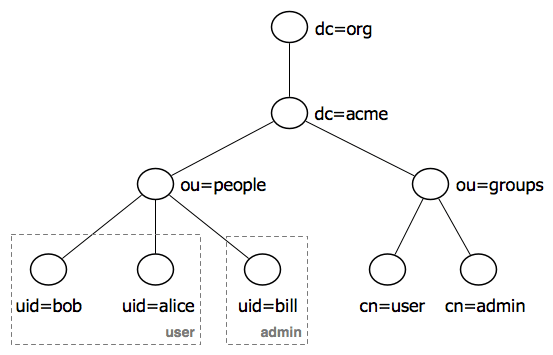
\includegraphics[width=1\linewidth]{imgs/acme_ldap.png}
    \caption{Schéma représentatif d'une hiérachie dans un annuaire}
    \label{fig:canal}
\end{figure}\\ \\
Un annuaire s'applique à un ou plusieurs DC \textit{Domain Component}, qui peuvent être un nom de domaine, un nom symbolique (e.g. DC = UPPA, ou DC = fr puis ce DC est rattaché à DC = univ-pau). Les DC sont la racine de l'arbre auquel vous souhaitez effectuer une recherche ou faire une affectation. 
\\ \\
À la suite de ces DC sont attachés des OU \textit{Organization Unit}, des groupes d'objets dans l'annuaire. Un exemple pourrait être la présence d'un OU pour les personnes de l'entreprise, puis dedans un OU \textit{Techniciens}, un OU \textit{Administrateurs}... L'agencement de l'arborescence se fait selon le besoin.
\\ \\
Ces OU sont composés de CN \textit{Common Name} qui sont les feuilles de l'arbre, l'élément final. Généralement des utilisateurs, des comptes... Peuvent aussi y être des UID \textit{User ID} pour globalement le même rôle, dépendemment de l'utilisation et des besoins.
\\ \\
Nous avons donc monté un serveur LDAP sous recommendations de l'enseignant pour ensuite monter l'arborescence voulue à l'aide de fichiers LDIF \textit{LDAP Data Interchange Format}. La recherche, l'ajout, la suppression ou la modificiation d'objet dans l'arbre se fait via l'écriture de fichiers LDIF, donnant une suite d'instruction à effectuer dans l'arbre.

\section{Aboutissants du module}

Par ce module nous avons appris comment monter un serveur LDAP, le gérer et par conséquence le comprendre. C'est un savoir essentiel en entreprise car extrêmement étant un outil largement présent et puissant.
    \renewcommand{\figurename}{}
\mychapter{R305 Chaîne de transmission numérique (27h)}{cap:r305}
\lhead{R305 Chaîne de transmission numérique (27h)}

\vspace*{0.2cm}%
      \large
      \href{\@orientadorPagina}{\color{black}Enseignant\\Mr. Angel Abénia}\\%
      \normalsize
\vspace*{0.5cm}%

Le module R305 a été abordé pendant la première période à l'IUT, son examen s'est déroulé sur la deuxième période pendant une heure. Ce module avait comme objectif la meilleure caractérisation des supports de transmission en étudiant de manière plus approfondie la transmission des signaux, donc leur étude.

\section{Caractérisation d'un canal de transmission}

Une mise en matière à ce module pourrait être les informations suivantes.
\begin{itemize}
  \item Pour communiquer, les appareils ont besoin d'avoir des informations à échanger, sinon ils n'auraient pas eu besoin d'avoir à communiquer.
  \item Les informations sont véhiculées par un signal, électromagnétique, optique, électrique ou hertzien.
  \item Un support, ou canal de transmission, est utilisé pour transmettre les signaux. Celui-ci est adapté selon la nature du support physique et le type de signal à transporter.
\end{itemize}

\begin{figure}[h]
    \centering
    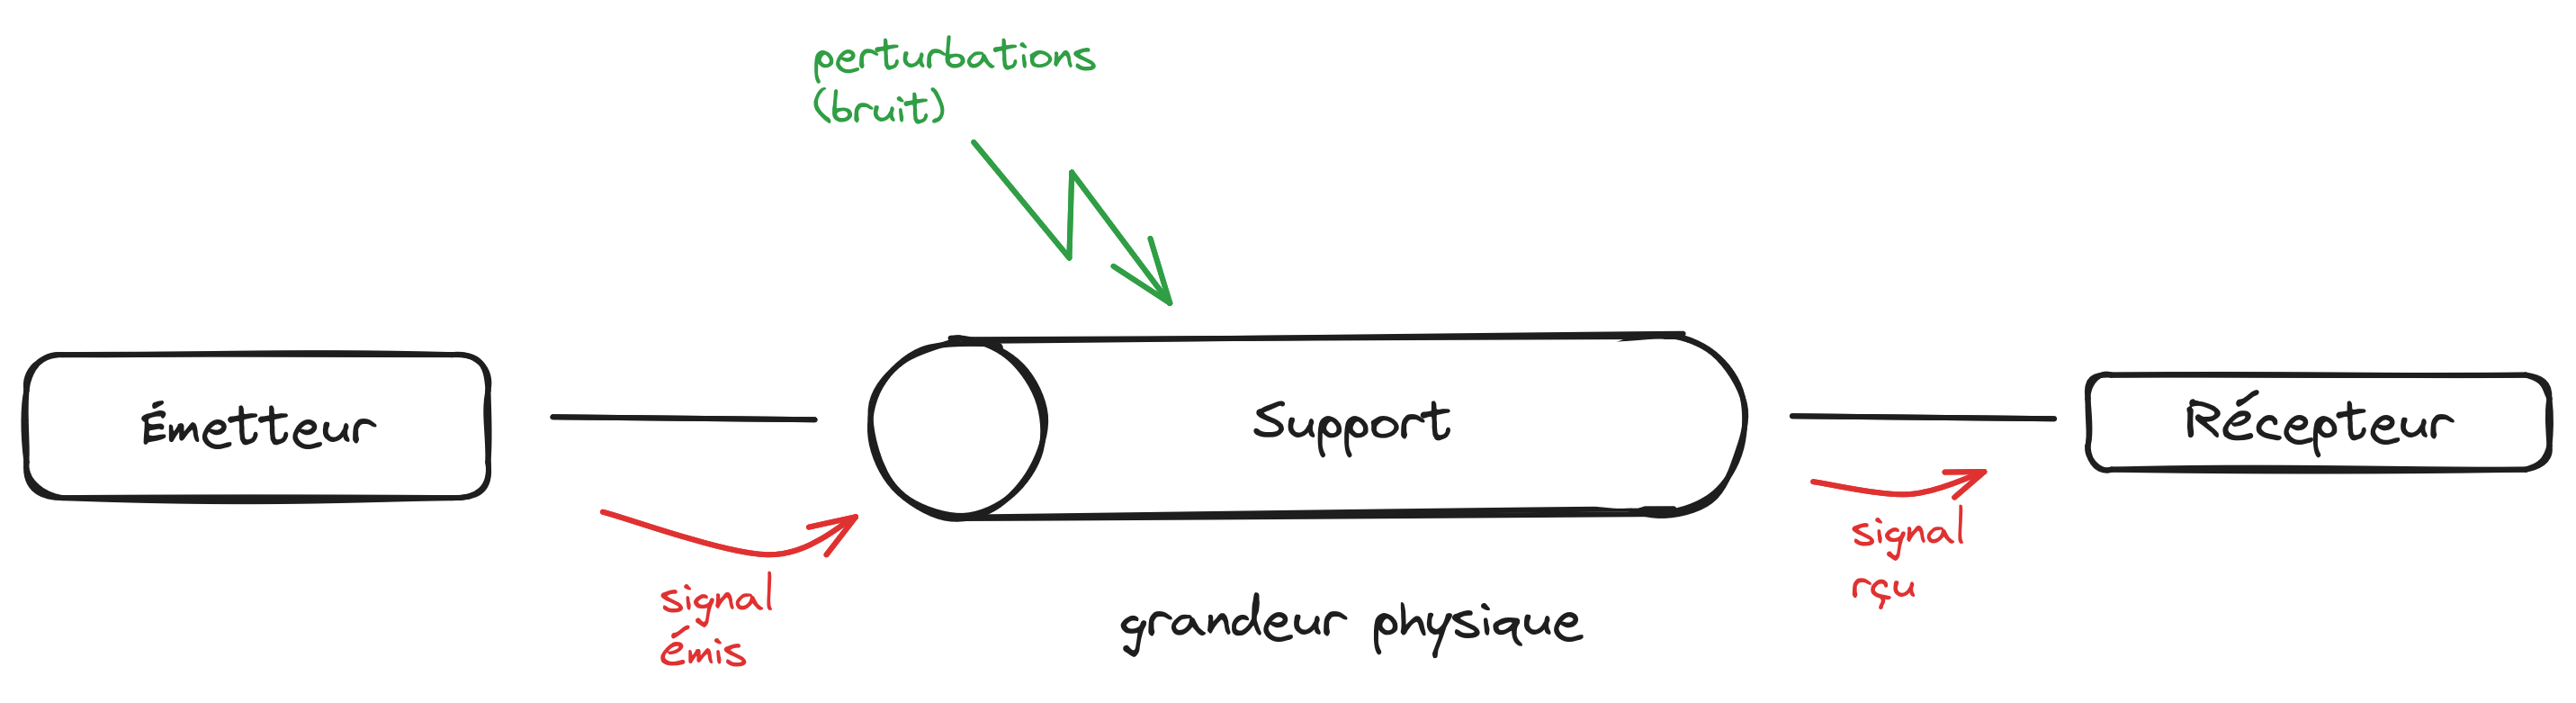
\includegraphics[width=1\linewidth]{imgs/support.png}
    \caption{Schéma représentatif d'un canal de transmission}
    \label{fig:canal}
\end{figure}

Un support de transmission admet une Bande passante \textbf{Bp}. Celle-ci est caractérisée par l'ensemble des fréquences que le canal permet de transporter. Ainsi que leur localisation dans l'espace des fréquences. Une bande passante admet donc une fréquence de début, une de fin, et une dernière centrale.
\\ \\
Bp de 100 Hz centrée sur 50 Hz. Soit Bp permet de transmettre toute fréquence dans l'intervale [0 Hz ; 100 Hz]
\\ \\
À leur dépassement à ses extrémités, le signal ne sera pas bien transmis; trop de dégradations seront appliquées pour les fréquences en dehors de la bande passante. Si nous pouvions avoir un canal de transmission parfait, avec aucune limite de bande passante et sans atténuation, alors le débit maximal théorique obtenable serait parfait aussi, outrepassant toute loi de la physique mais utile pour des calculs.
\\ \\
Ainsi, un canal de transmission avec une meilleure bande passante permet un meilleur débit binaire théorique : e.g. avec la fibre optique et une paire torsadée. Le signal "ne va pas plus vite", la vitesse de l'électricité dans un conducteur étant relativement proche de celle de la lumière dans du silice, mais la bande passante permise par le changement de support permet un meilleur débit, par la fibre moins d'atténuation, facilitant l'élargissement de la bande passante.
\\ \\
Dans la caractérisation de la chaîne de transmission du monde du numérique, nous avons rappelé le principe de liaison synchrone et asynchrone (synchronisation des horloges ou resynchronisation du front de décision à chaque information). Nous avons aussi revu le principe de débit binaire maximal théorique (brut), et celui dit "net" à l'utilisation - après toutes les informations nécessaires à la transmission des données ajoutées pour assurer sa transmission (dans les entêtes et queues des couches des protocoles).
\\ \\
Dans la caractérisation d'un signal, nous avons vu l'apparition des zones de décision pour différencier les états significatifs d'un signal. Pouvant se traduire par la plage de décision permise pour définir si l'on peut différencier un état significatif du signal (codant une information), pouvant laisser place à une zone d'incertitude. La place de décision doit toujours être inférieure au temps d'un état, sinon possibilité de confusion.

\begin{figure}[h]
    \centering
    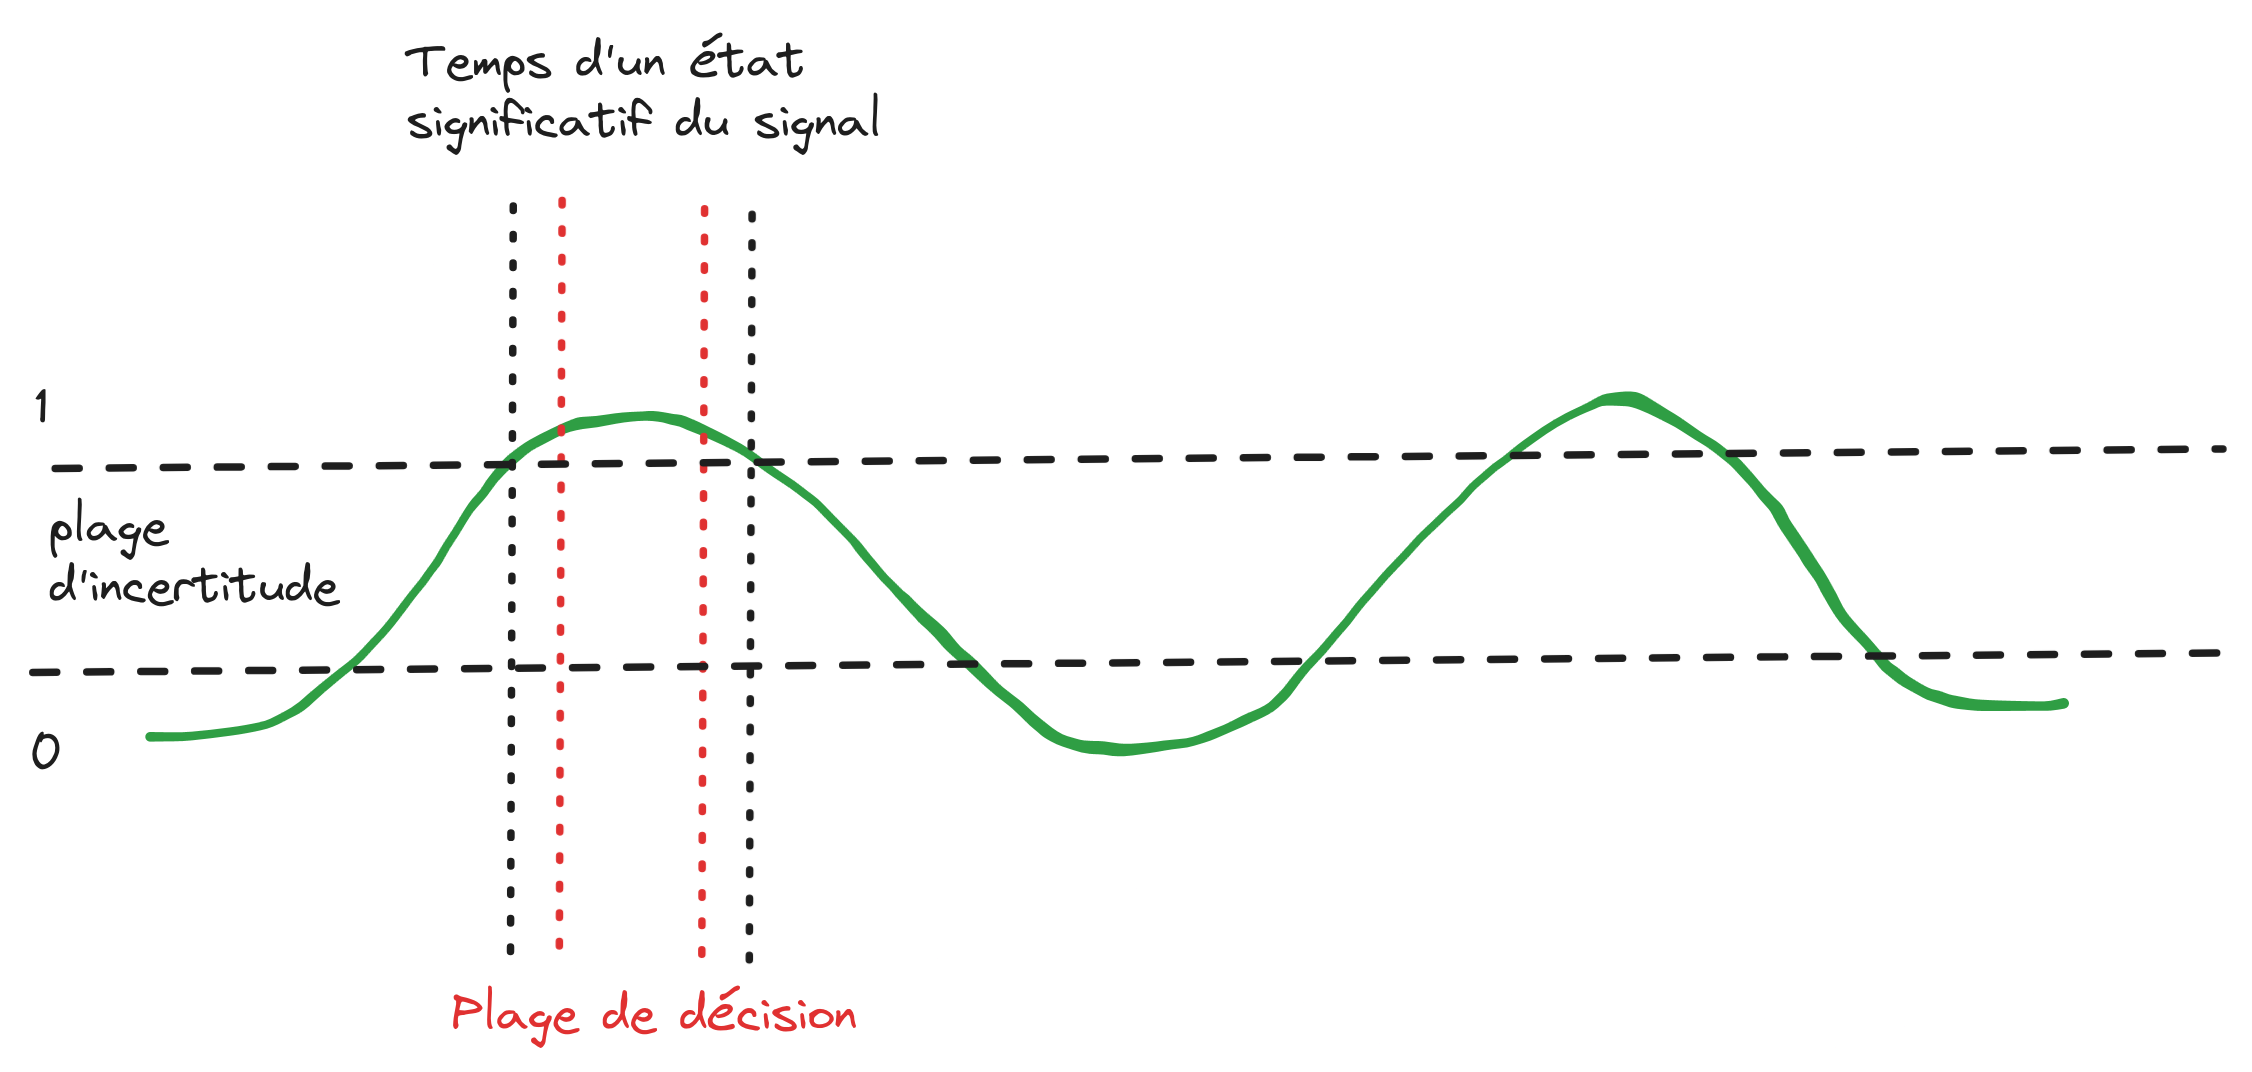
\includegraphics[width=1\linewidth]{imgs/td.png}
    \caption{Schéma représentatif de la décision d'un état pour une sinusoïde simple, ou "comment définir l'état d'un signal"}
    \label{fig:td}
\end{figure}

Par ce schéma, on peut en ressortir que si une plage de décision est trop large comparée au moment d'un symbole (état significatif d'un signal) : on peut confondre un état pour un autre. Il s'agit de l'interférance inter-symbole, ici représenté par deux états électriques +A -A (A pouvant être négatif). L'intérêt est de bien configurer les seuils de décisions (encadrement des valeurs du signal - plage d'incertitude) et les temps de décisions (plage de décision d'un moment).
\\ \\
Un autre moyen plus simple de mettre en évidence l'interférance inter-symbole est de diagramme de l'oeil. Dans celui-ci sont défini tous les passages possibles des états.

\begin{figure}[h]
    \centering
    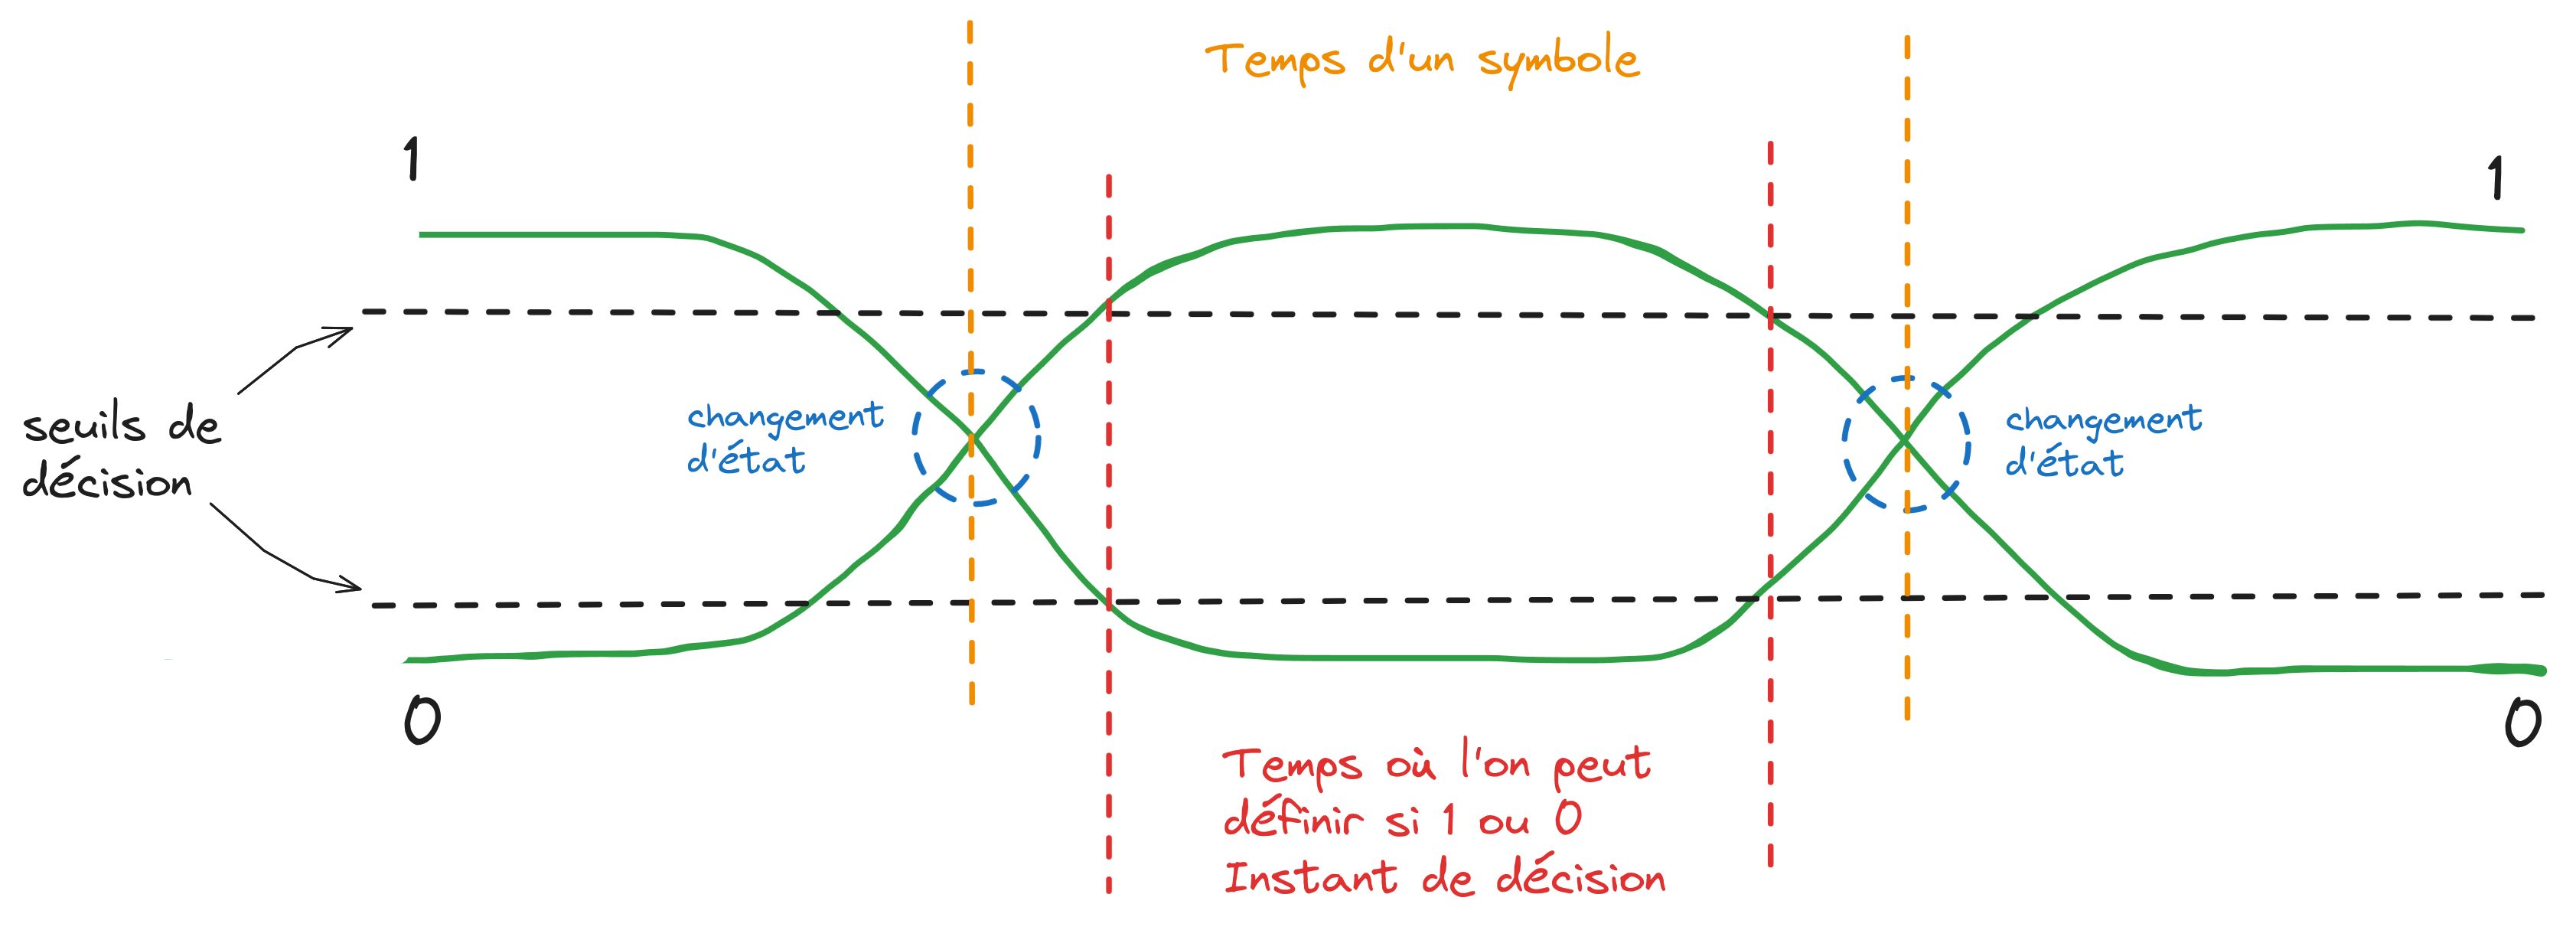
\includegraphics[width=1\linewidth]{imgs/seuils.png}
    \caption{Introduction au diagramme de l'oeil par identification des états d'un signal carré sans bruit (très fin)}
    \label{fig:seuils}
\end{figure}

Le temps où l'on peut définir si l'état est à 0 ou 1 ne peut être plus grand ou égale qu'à celui des symboles, sinon interférence inter-symbole. Le temps d'un symbole commence dès le changement du précédent état. Si l'instant de décision n'est pas correcte, deux choix pour atteindre les seuils si on ne peut pas les modifier : diminuer le débit pour faire rentrer le signal dans leur intervale, ou augmenter la bande passante - en changeant de canal de transmission.
%\\ \\
%Nous avons fait la différence entre le débit binaire brute théorique attégnable, et celui reçu après informations rajoutées aux données envoyées (destination dans un réseau, gestion de sessions, encapsulation de protocoles...) dans des entêtes et/ou des queues.
\\ \\
Nous pouvons changer le débit en conservant une bande passante correcte en jouant sur la valence du signal. En conservant la même fréquence, nous pouvons moduler le signal en amplitude ou en phase afin d'avoir davantage de symboles. La limite de cette pratique nous est donné par les travaux de Mr. Shanon que nous avons étudié, fixant que la valence se limite à ce que permet le rapport signal sur bruit, pour distinguer tous les états.
\\ \\
Nous avons aussi repris les travaux de Mr. Nyquist en intégrant ses critères pour définir la capacité d'un canal, soit sa bande passante maximale dans le domine théorique et physique. Nous avons notamment démontré la différence entre ces deux en travaux pratiques.
\\ \\
Si le débit binaire augmente, la bande passante aussi, sinon interférence entre les symboles. Pour contrer ceci soit augmenter la bande passante, soit réduire le débit, soit jouer sur les seuils et les instants de décision. D'autres états peuvent être introduits par modulation, à question que ceux-ci puissent être distingués, donc pas limités par le rapport entre le niveau de puissance du signal et celui du bruit.

\section{Fiabilisation d'une transmission}

La fiabilisation d'une transmission peut se caractériser par sa capacité à transmettre un message selon des circonstances données. Ainsi, des mécanismes de contrôle d'erreurs sont instaurés avec une demande de ré-émission par exemple. Le choix du type de transmission est aussi important, sa modulation. Dans cette partie nous avons abordé les codecs et nous avons étudié les types de modulation (manchester, NRZ...).
\\ \\
Certains types de modulations permettent une meilleur résistance au bruit, notamment ceux par phase vu diagramme de constellation. Chacun code le signal comme il le souhaite, le temps et les chercheurs sont par exemple passés du codage NRZ \textit{non-return-to-zero} à du PSK \textit{Phase-shift keying} ou du QAM \textit{quadrature amplitude modulation} toujours utilisés aujourd'hui. Leur largeur de spectre pour les mêmes informations envoyées changent aussi, pareil que pour son emplacement dans un spectre d'amplitude (lobe principal centré sur 0 Hz pour ceux qui ne modulent pas en fréquence...).

\section{Aboutissants du module}

Nous avons approfondi nos connaissance dans les supports de transmissions qui nous servent aujourd'hui. Nous pouvons les caractériser correctement pour montrer une infrastructure, nous pouvons les diagnostiquer dans nos domaines de compétences. Nous comprenons désormais comment circule un signal dans la "chaine du transmission du numérique", son histoire et son arrivée au monde moderne.
    \renewcommand{\figurename}{}
\mychapter{R307 Réseaux d'accès (24h)}{cap:r307}
\lhead{R307 Réseaux d'accès (24h)}

\vspace*{0.2cm}
      \large
      \href{\@orientadorPagina}{\color{black}Enseignant\\Mr. Yannick Lespine}\\
\vspace*{0.5cm}

Enseignement délivré sur la première période à l'IUT. Ce module avait pour objectif de nous faire apprendre les technologies des réseaux d'accès des FAI \textit{Fournisseur d'Accès Internet}. Celui-ci est lié au module R302 et les réseaux d'opérateurs, aussi appelés réseaux backbone. Ce module a un fort coefficient dans la deuxième compétence télécommunications. Nous y avons étudié en profondeur les technologies xDSL, et appliqué certains principes réseaux comme le DHCP, le NAT et d'autres.

\section{Apprentissage théorique des réseaux à technologie xDSL}

Lors des cours et des travaux dirigés, nous avons intégré le fonctionnement des réseaux d'accès à technologie xDSL \textit{Digital Subscriber Line}. Basés sur le réseau téléphonique déjà existant, les technologies xDSL avaient comme objectif de l'utiliser pour raccorder des abonnées à Internet, en plus d'accéder à la téléphonie. De là sont nés l'ADSL \textit{Asymetric DSL} GDMT, 2 et 2+ ou encore la VDSL \textit{Very high-speed Digital Subscriber Lines}.
\\ \\
L'ADSL est la technologie que nous avons le plus abordé. Celle-ci est présente dans sa plus ancienne version, GDMT, jusqu'à la dernière l'ADSL2+. Ces deux possèdent des spectres conservant la déontologie des spectres de réseau ADSL : une bande passante pour le POTS \textit{Plain Old Telephone Service (la téléphonie)}, une autre pour le flux sortant et une plus grande pour le flux rentrant (car abonné consommateur de services sur Internet, pas producteur).

\begin{figure}[h]
    \centering
    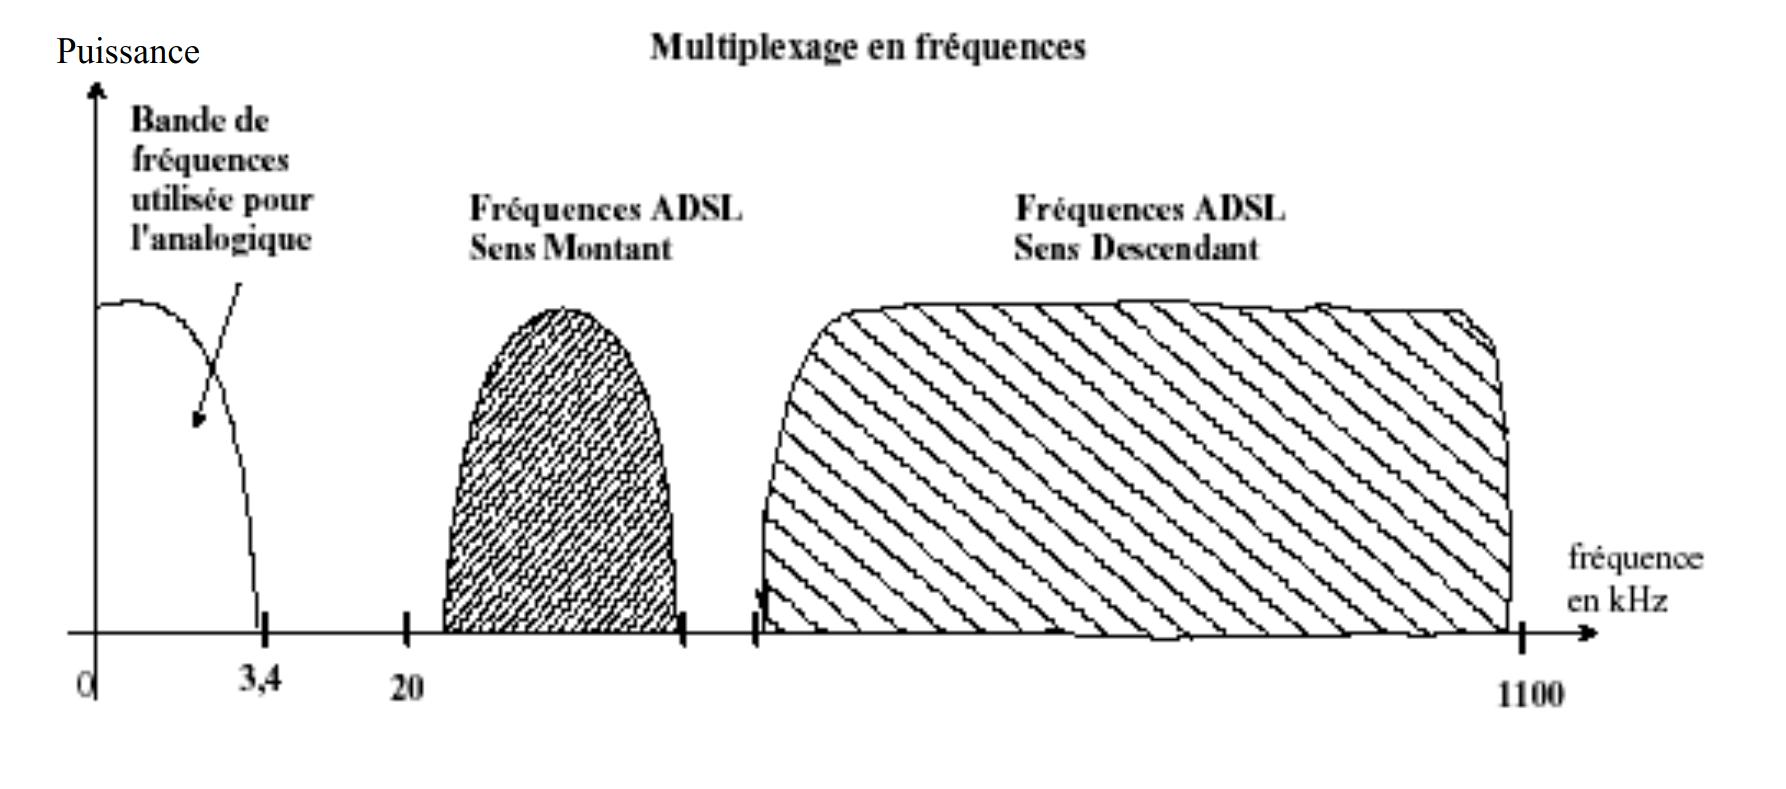
\includegraphics[width=1\linewidth]{imgs/tmp_adsl.jpg}
    \caption{Spectre d'amplitude d'un lien ADSL}
    \label{fig:tmp_adsl}
\end{figure}

L'ADSL utilise une modulation dans son signal pour tirer le meilleur débit possible de ses bandes passantes. Nous avons revu les types de modulation, sans aborder dans les détails la modulation DMT \textit{Discrete MultiTone} de l'ADSL. Nous avons aussi confirmé que le débit maximal pratique était définit par la distance qui nous reliée à l'équipement de l'opérateur. En effet, le support étant une paire de cuivre torsadée, celle-ci se comporte comme une résistance au passage du courant : elle augmente sa résistivité par la distance et le courant traversé. Les fréquences qui composent le signal reçoivent une atténuation de plus en plus forte proportionnellement à la distance, ce qui diminue leur valence, et donc le débit qu'elles peuvent faire transiter.
\\ \\
La modulation est gérée d'un côté par un modulateur et de l'autre par un démodulateur. Ce mécanisme fonctionne pour une communication dans un sens (celui qui envoie n'est pas celui qui reçoit). Pour que les deux côtés puissent envoyer et recevoir des informations, ont été conçu les modems - abrévation pour modulateur/démodulateur. L'équipement chargé de cette action chez le FAI est le DSLAM \textit{Digital Subscriber Line Access Multiplexer} qui s'occupent de rattacher les équipements abonnés au réseau backbone opérateur pour accéder à internet, et le modem chez le client pour envoyer des informations selon la même modulation au DSLAM, et démoduler celles reçues.
\\ \\
Nous avons aussi beaucoup étudié les couches protocolaires, comme le fonctionnement du protocole ATM \textit{Asynchronous Transfer Mode} et ses cellules, aisni que ses protocoles de couches supérieures. Nous avions ainsi toutes les informations nécéssaires, et plus, pour comprendre le type de topologie ci dessous.

\begin{figure}[h]
    \centering
    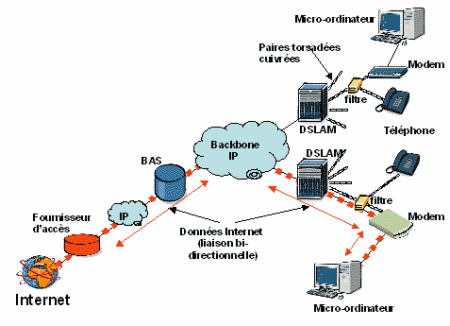
\includegraphics[width=1\linewidth]{imgs/tmp_adsl2.png}
    \caption{Schéma d'une liaison opérateur FAI et abonné en ADSL}
    \label{fig:tmp_adsl2}
\end{figure}

Le BAS \textit{Broadband Access Server} est un serveur permetant l'authentification des abonnées par l'utilisation de protocoles comme le PPPoE \textit{Point-to-Point Protocol over Ethernet} sur la couche ethernet ou le PPPoA \textit{PPPo ATM} sur la couche ATM. Auquel cas n'importe qu'elle personne, sans abonnement, pourrait se rattacher au DSLAM par un port téléphonique raccordé et récupérer une adresse IP pour avoir accès à Internet. Ce serveur authentifie les abonnées auprès de l'opérateur, permettant la réception d'une adresse IP et leur accès à Internet \& aux services globales de l'opérateur.

\section{Projet d'étude d'un réseau d'accès ADSL}

Lors des travaux pratiques, nous avons pu mettre en place et caractériser un réseau à technologie ADSL. À l'issue de ce projet, nous avions un rapport globale à rendre et une présentation à soutenir. Les travaux pratiques constituent la moitié du temps consacré à ce module (12h).
\\ \\
Les premières séances de ce projet étaient dédiées à la prise en main des équipements mis à disposition et à la compréhension l'infrastructure de la salle. Ainsi, nous avons pris en main un modem et routeur Zyxel VMG1312-B10D pour l'équipement abonnée, un DSLAM ADSL IES 1000 côté opérateur, un testeur de ligne xDSL SUNRISE TELECOM MTT LITE DSL, des routeurs Cisco 2901 pour simuler l'arrière du réseau opérateur, et le réseau de la salle.
\\ \\
Nous avons abordé des notions plus en profondeur qu'en cours, en poussant notre étude pour comprendre le fonctionnement d'outils ou de notions annexes (diaphonie, synchronisation ADSL...). Nous avons lors de ce projet caractérisé une ligne ADSL via le testeur de ligne et interprété ses valeurs. Nous avons configuré les équipements de réseaux conformément aux apprentissages demandés (côté opérateur et abonné) afin de comprendre les différents types de topologies, pourquoi certaines comme celle en pont ne sont plus utilisés... Des protocoles, couches ou notions annexes ont aussi été abordé comme le DHCP dans le LAN et côté opérateur, la gestion de l'authentification par le protocole PPP, monter - caractériser \& différencier les types de NAT...
\\ \\
Le rapport de ce projet est disponible sur \href{https://karuta.univ-pau.fr/karuta-backend/resources/resource/file/1e82435e-9d2d-11ee-a8e6-aae0820000f2?lang=fr&timestamp=1706858357601https://karuta.univ-pau.fr/karuta-backend/resources/resource/file/1e82435e-9d2d-11ee-a8e6-aae0820000f2?lang=fr&timestamp=1706858357601}{Karuta}, les notes et le coefficient de ce module en annexe.

\section{Aboutissants du module}

Par ce module et particulièrement son projet intégratif, nous avons pu monter et étudier un réseau opérateur-abonné. Enseignement extrêmement intéressant, regroupant réseaux et télécommunications pour nous faire apprendre les différentes technologies les composants encore aujourd'hui. Les appliquer sur des équipements particuliers a aussi été très enrichissant pour l'utilisation d'outils tiers.
    \renewcommand{\figurename}{}
\mychapter{R308 Consolidation de la programmation (27h)}{cap:r308}
\lhead{R308 Consolidation de la programmation (27h)}

\vspace*{0.2cm}
      \large
      \href{\@orientadorPagina}{\color{black}Enseignant\\Mr. Manuel Munier}\\
      \normalsize
\vspace*{0.5cm}

Module portant sur la programmation avec le language Python, nous y avons revu les bases de la programmation séquentielle. L'exercice tendait à montrer que la lecture séquentielle d'un document (ligne par ligne), même en créant des fonctions ou en utilisant les méthodes des objets de base de Python; n'était pas forcément pas la meilleure manière de programmer selon le cas d'usage. Ainsi, nous avons abordé la POO \textit{\textbf{Programmation Orientée Objet}}.

\section{Introduction à la programmation orientée objet}

La POO, ou \textit{Programmation Orientée Objet}, est une autre approche de la programmation (paradigme), une manière d'aborder le code différemment. Celle-ci se caractérise par l'utilisation d'objets : un agencement de données et de code (une structure); pour définir un ensemble d'éléments réutilisables. Ainsi, pour un objet donné, plusieurs \textbf{instances} de celui-ci peuvent être générées. Chaque instance reprenant l'agencement du code défini. Les instances récupère le code et les données qui le constitue.
\\ \\
Les objets peuvent être comparés à du papier calque, reproduisant leur structure sur chaque instance pour faciliter leur génération, sans avoir à les régénérer à chaque fois.
\\ \\
Des fonctions peuvent être créées pour chaque objets, alors appelées des \textbf{méthodes}. Pour une méthode \verb|afficher_age(self)| crée de l'objet \verb|Personnes|, chaque instance pourra être appelée de la sorte : \verb|print(julien.afficher_age())| pour afficher l'âge d'une personne.
\\ \\
La POO, selon les cas d'usages, est une approche beaucoup plus propre pour agencer son code. Si l'on en trouve l'utilité, la POO est un outil très puissant pour répliquer ra

\section{Cas d'usage de la POO}

La POO est extrêmement utile pour s'assurer que chaque élément possède le même paterne, et que chaque instance puisse être appelée de la même manière. La POO est simple, et facilement intégrable sans son code une fois que nous en avons compris le fonctionnement et son utilisation dans Python.
\\ \\
Un cas d'usage générique pourrait être : \textit{Considérons l'objet "Personnes". Chaque instance de l'objet "Personnes" possédera le même paterne : un nom, un prénom, un âge... Celles-ci partageront aussi les mêmes méthodes} \verb|afficher_prenom()| \textit{et} \verb|afficher_nom()| \textit{qui retourneront leurs informations respectives, pour au mieux les intégrer à votre code (avec des conditions...).}\\- cette mise en situation provient de moi.

\section{Utilisation avancée}

 Un objet peut \textbf{hériter} des propriétés d'un autre objet, si besoin d'instancer deux types d'objets très similaires : pas besoin de créer deux fois deux objets similaires; juste de créer un objet global et d'en créer un deuxième héritant des propriétés du premier en modifiant certaines informations en les écrasant ou en les rajoutant.
 \\ \\
 Une méthode peut retourner une information d'une instance ou la modifier.
 \\ \\
 La POO est souvent utilisée pour la structuration avancée de données : arbre binaire de recherche notamment, notamment dans les cas où chaque donnée conservent globalement le même paterne.

 \section{Aboutissants du module}

 Ayant déjà abordé la POO auparavant, j'ai pu cette fois-ci l'intégrer dans des exercices plus complexes pour y découvrir des cas d'usages particuliers, que je n'aurais probablement pas soupçonné sans eux. Module très enrichissant pour sa manière d'aborder le code, son cheminement de pensées à avoir.
 \\ \\
 Tous les exercices que j'ai effectué, avec leur sujet, sont retrouvables sur mon \href{https://github.com/xeylou/r308}{Github}.
    \renewcommand{\figurename}{}
\renewcommand{\tablename}{}
\mychapter{R310 Gestion d'un système de bases de données (10h30)}{cap:r310} 
\lhead{R310 Gestion d'un système de bases de données (10h30)}

\vspace*{0.2cm}
      \large
      \href{\@orientadorPagina}{\color{black}Enseignant\\Mr. Stéphane Mascaron}\\
      \normalsize
\vspace*{0.5cm}

Module le plus court abordé lors de cette première période. Celui-ci abordait les types de bases de données, leurs cas d'usage et leurs spécificités. Après un apprentissage théorique de l'histoire derrière leur utilisation, et de comment en choisir une en adéquation avec nos besoins; nous avons pris en main la BDD \textit{Base De Données} NoSQL MongoDB.

\section{Caractérisation des bases de données les plus courantes}

Après l'utilisation de fichiers texte pour le stockage d'informations, les bases de données ont émergées pour une utilisation plus sérieuse. Celles-ci ont évoluées au cours du temps, passant des bases de données relationnelles dites SQL \textit{Structured Query Language} à d'autres dites en graphes, en objet, ou en document...
\\ \\
Les bases de données peuvent être regroupées en deux catégories selon leur paradigme : les ACID \textit{Atomic, Consistent, Isolation, Durable} et les BASE \textit{Basically Available, Soft state, Eventual consistent}. Les premières bases de données étaient des relationnelles, respectant les principes d'ACID. Les plus récentes ont abandonnées ce modèle pour respecter les principes BASE.
\\ \\
Pour résumer les principes d'ACID, ils impliquent que pour une base de données, répartie sur plusieurs serveurs ou non, celle-ci doit retourner les mêmes valeurs chaques mêmes requêtes. Ce qui peut être problématique question performances, certains logiciels fonctionnent par ailleurs très bien sans des réponses exactes (sur Instagram, il n'est pas si grave que vous voyez 15'241 "j'aime" au lieu de 15'314).
\\ \\
L'\textbf{atomicité} suggère que chaque transaction est faite en entier ou pas du tout, la \textbf{consistance} que toutes les données écrites respectent les contraintes d’intégrités et que l’état de la base de données reste toujours valide, l'\textbf{isolation} qu'un échange en parallèle donne toujours le même résultat qu’un échange en série et la \textbf{durabilité} qu'une fois les données écrites elles le restent.
\\ \\
Les principes BASE ont vu émerger quatres grands types de bases de données : les BDD suivant le modèle d'une clé - une valeur pour de la grande sauvegarde sans structure, les BDD suivant la théorique des graphs pour faire des liens entre des objets; omniprésent comme BDD derrière les réseaux sociaux pour faire des liens entre des personnes, ceux à document suivant permettant un modèle extrêmement flexible de données, et celles à colonnes avantageuses pour de la corrélation de données. Ces bases de données sont aussi appelées NoSQL, en opposition aux bases de données relationnelles SQL/ACID.
\\
\begin{table}[h]
\begin{tabular}{|l|l|l|l|l|l|}
\hline
Modèle     & Performance & Évolutivité & Flexibilité & Complexité & Fonctionnalité    \\ \hline \hline
Clé/Valeur & Élevée      & Élevée      & Élevée      & Aucune     & Variable (aucune  \\ \hline
Colonne    & Élevée      & Élevée      & Modérée     & Faible     & Minimale          \\ \hline
Document   & Élevée      & Variable    & Élevée      & Faible     & Variable (faible) \\ \hline
Graphe & Variable & Variable & Élevée & Grande & \begin{tabular}[c]{@{}l@{}}Théorie des graphs\end{tabular} \\ \hline
\end{tabular}
\caption{Tableau comparatif des BDD NoSQL}
\end{table}

\section{Prise en main de MongoDB}

Une fois l'apprentissage théorique terminé, nous avons pris en main une base de donnée NoSQL orientée documents, MongoDB. En raison, nous avions déjà eu au semestre dernier un module dédié à l'apprentissage et la prise en main du language SQL.
\\ \\
MongoDB stocke des données au format BSON (JSON mais au format binaire). La structure de MongoDB se caratérise par ses trois couches.

\begin{itemize}
  \item Des \textbf{Databases} qui contiennent des \textbf{Collections}
  \item Chaque \textbf{Collection} contient des \textbf{Documents}
  \item Chaque \textbf{Document} est au format BSON, utilisé JSON, et contient des \textbf{Propritétés} (clé/valeur)
\end{itemize}

MongoDB est une base de donnée \textbf{sans schéma}, c'est-à-dire qu'un document peut avoir la structure qu'il souhaite. À contrario de SQL qui sont définis et obligatoires. Donc chaque collection peut avoir une forme différentes, leurs documents étant de compositions dissemblantes au fur et à mesure des insertions \& suppressions. La structure de donnée est donc assouplie, pouvant rajouter les types de données qu'on souhaite comparé aux SQL.
\\ \\
MongoDB apporte une souplesse impréssionnante par la structure de ses documents et une rapidité accrue. Cependant cela se paye par une corrélation des données (on ne peut pas effectuer les mêmes actions partout, on contrôle moins les données).
\\ \\
Dans sa forme la plus basique, MongoDB fonctionne comme un serveur simple avec un \textbf{mongo shell} pour contacter la Database hébergée. Il supporte le scaling horizontal (ajout de serveur) pour distribution de charge ou accessibilité multi-site avec synchronisation. L'équipe développant MongoDB a aussi mis en place une application WEB pour une visualisation des collections et documents d'un plus haut niveau.
\\ \\
Le mongo shell peut être utilisé selon la forme suivante : \\ \verb|<database>.<collection>.<fonction()>|, où la fonction est l'action demandée sur la collection. Par exemple, pour la base de donnée "db", et la collection exercices, nous pouvons lire les données d'une collection avec la fonction find : \verb|db.exercices.find()|. Nous avons été guidé en travaux pratiques pour prendre en main le mongo shell, pour des actions de bases sur une base de données MongoDB.
\\ \\
Pour l'administration de la base de donnée, pas que des appelles, l'utilitaire \textbf{mongosh} peut être utilisé. Exemple de commande pour lancé le shell de MongoDB avec le compte \verb|root| et le mot de passe \verb|azerty| sur la database admin (qui répertorie les utilisateurs admin) : \\ \verb|mongosh -u "root" -p "azerty" --authenticationDatabase "admin"|.

\section{Aboutissants de l'apprentissage}

Grâce à ce module, nous avons pu apprendre à différencier les types de bases de données et à savoir laquelle choisir selon nos besoins. Nous avons aussi vu l'administration et l'utilisation d'une base de donnée MongoDB. Toutes mes manipulations sur ce module sont retrouvables sur mon \href{https://github.com/xeylou/r310}{Github}. J'ai aussi créer un script d'installation automatisé d'une base de donnée MongoDB sur Debian12 toujours sur mon \href{https://gist.github.com/xeylou/ca01e4f17e6bbcc5e8bba042b37771d3}{Github}.
    \renewcommand{\figurename}{}
\mychapter{R312 ExpreComm professionnelle 3: savoir collaborer (12h)}{cap:r312} 
\lhead{R310 ExpreComm professionnelle 3: savoir collaborer (12h)}

\vspace*{0.2cm}
      \large
      \href{\@orientadorPagina}{\color{black}Enseignant\\Mme. Marilyne Carretier}\\
      \normalsize
\vspace*{0.5cm}

Dans ce module, nous devions développer notre savoir communiquer à travers d'exercices collectifs. À savoir des exercices de communication avec un groupe pour monter un projet en une heure puis le présenter, ou bien un exercice de communication à d'autre groupe pour les convaincre d'une idée.
\\ \\
Les exercices se ressemblaient dans leur fond : savoir communiquer avec un groupe pour se mettre en accord pour l'agencement d'une salle de restaurant, pour présenter une idée dans un domaine donné ou autre. Ces exercices avaient pour but de nous mettre en relation, savoir communiquer son idée et écouter celles des autres pour céder son idée ou agrémenter celles des autres.
\\ \\
Plusieurs jeux de rôles ont été fait pour montrer notre capacité à communiquer notre devant un groupe de personnes. Mises en situation, embauche, compréhension de gestion de situation... Le but était aussi de trouver une formulation pour faire valoir notre idée, pour que les personnes soient convaincus de son utilité.
    \mychapter{Annexes}{cap:annexes}
\lhead{Annexes}

Regroupement des documents servant à l'appui des éléments cités précédemment. Pouvant être de toutes formes (images, blocs de texte, photos...).

\section{Cahier des charges supervision}

Cahier de charges supervision

La recherche de solution applicative de supervision devra se base au
minimum sur deux applications pour avoir une comparaison objective.

Voici les fonctionnalités souhaitées~:

\ul{Serveurs Proxy}

L'utilisation de \textbf{SERVEUR PROXY} pour ne pas avoir un seul
serveur qui se charge de l'ensemble de vérifications de sonde.

\ul{DASHBOARD}

Un \textbf{DASHBOARD UNIQUE} qui inclut l'ensemble des serveurs de
supervision.

\ul{DASHBOARD TV}

Un \textbf{DASHBOARD} pour la télé qui liste les notifications de la
plus récente a la plus ancienne. (Comme celle que l'on a actuellement.)

\ul{Type de contrôles}

L'application devra gérer les contrôles \textbf{PASSIF} et
\textbf{ACTIF} et la prise en charge des contrôles via \textbf{SNMP}.

\ul{Type de paramétrages}

La possibilité de configurer les hosts via l'interface graphique et via
les fichiers de configuration.

Exemple~: sur l'ancienne supervision on créer un fichier de conf par
client.

\ul{Notifications}

Les notifications devront être effectuées par mail et par SMS tout en
ayant une gestion des utilisateurs et des groupes (possibilité
d'intégrer la solution à notre serveur d'SMS)

Déplacer le GSM dans le bureau ADITU de Pulseo pour une meilleur
couverture réseau (prévoir onduleur + switch mangeable)

\ul{Accès restreint client}

Donner la possibilité à certains clients de visionner leur supervision
en lecture et d'être alerté par mail.

\ul{Graphique}

Côté graphique, il serait bien que la solution puisse avoir la
possibilité d'inclure les graphiques comme fait Cacti pour éviter
d'avoir 2 solutions.

\begin{itemize}
\item
  Graphique réseau
\item
  Graphique volumétrie disque pour voir l'évolution du stockage
\item
  Graphique mémoire ou CPU
\end{itemize}

\ul{Tarif}

Open source gratuit

% \begin{figure}[H]
%     \centering
%     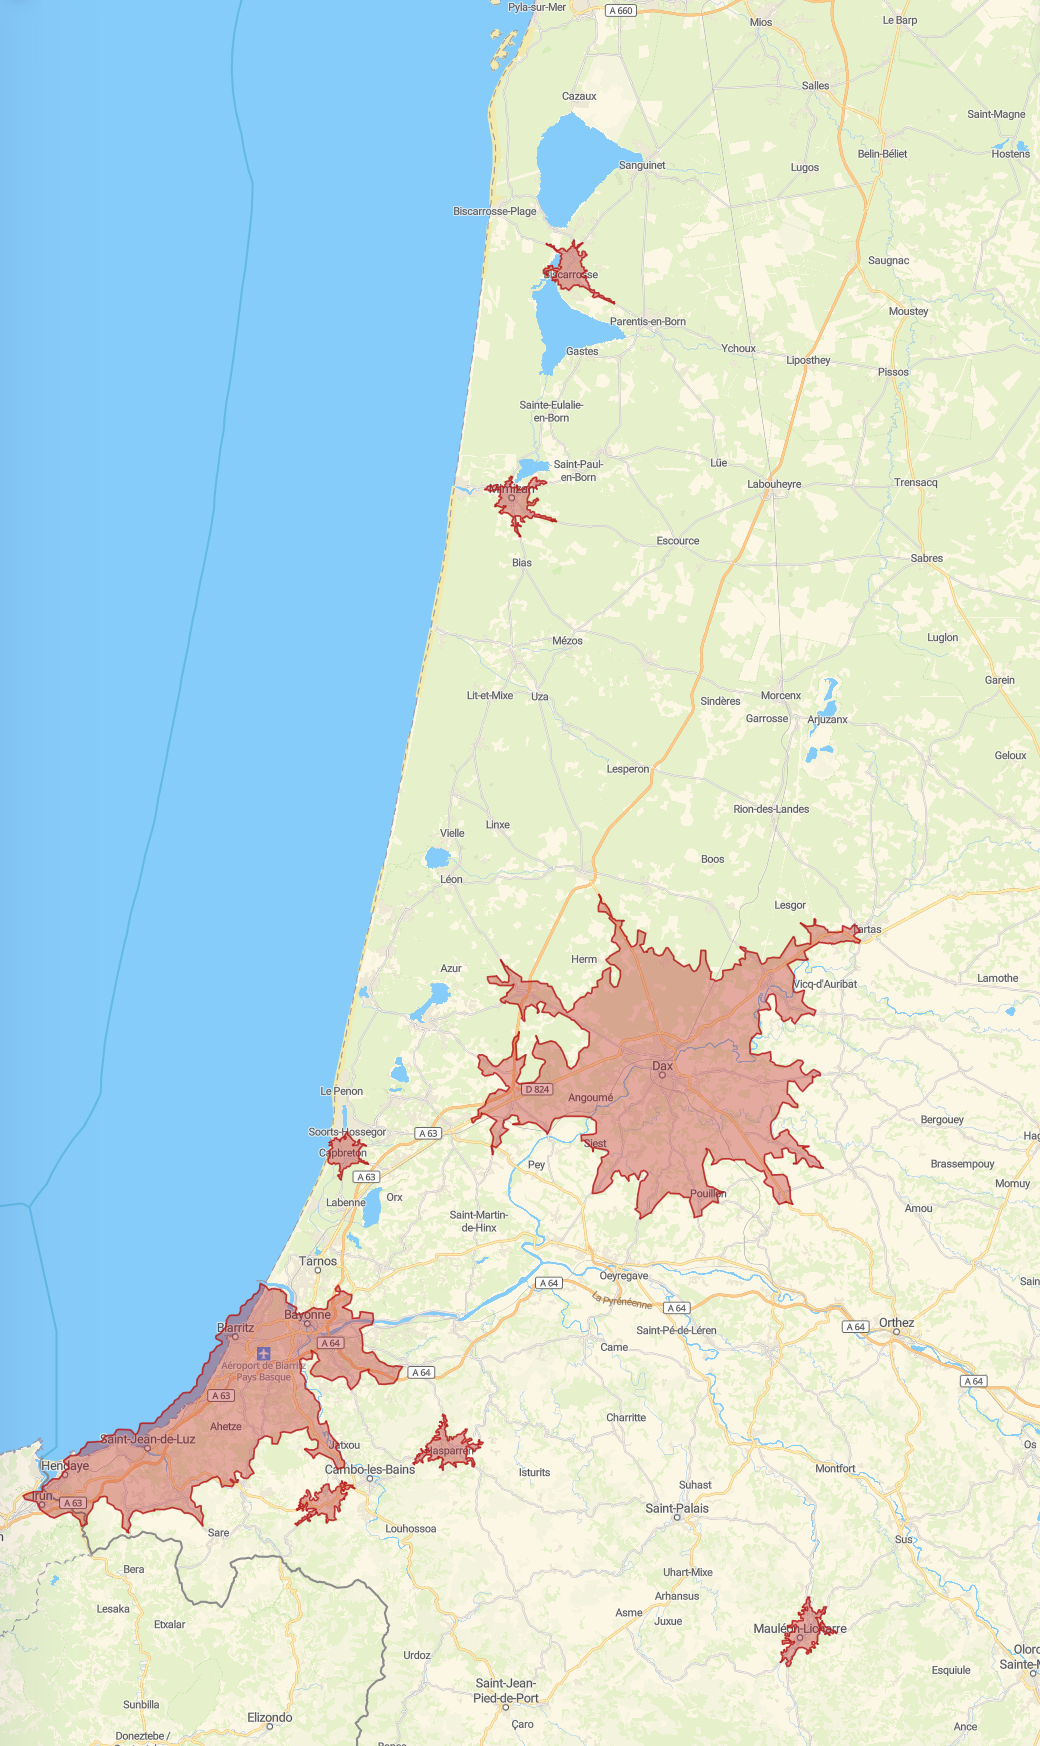
\includegraphics[width=\textwidth - \textwidth / 5]{zone_chalandise_aditu.png}
%     %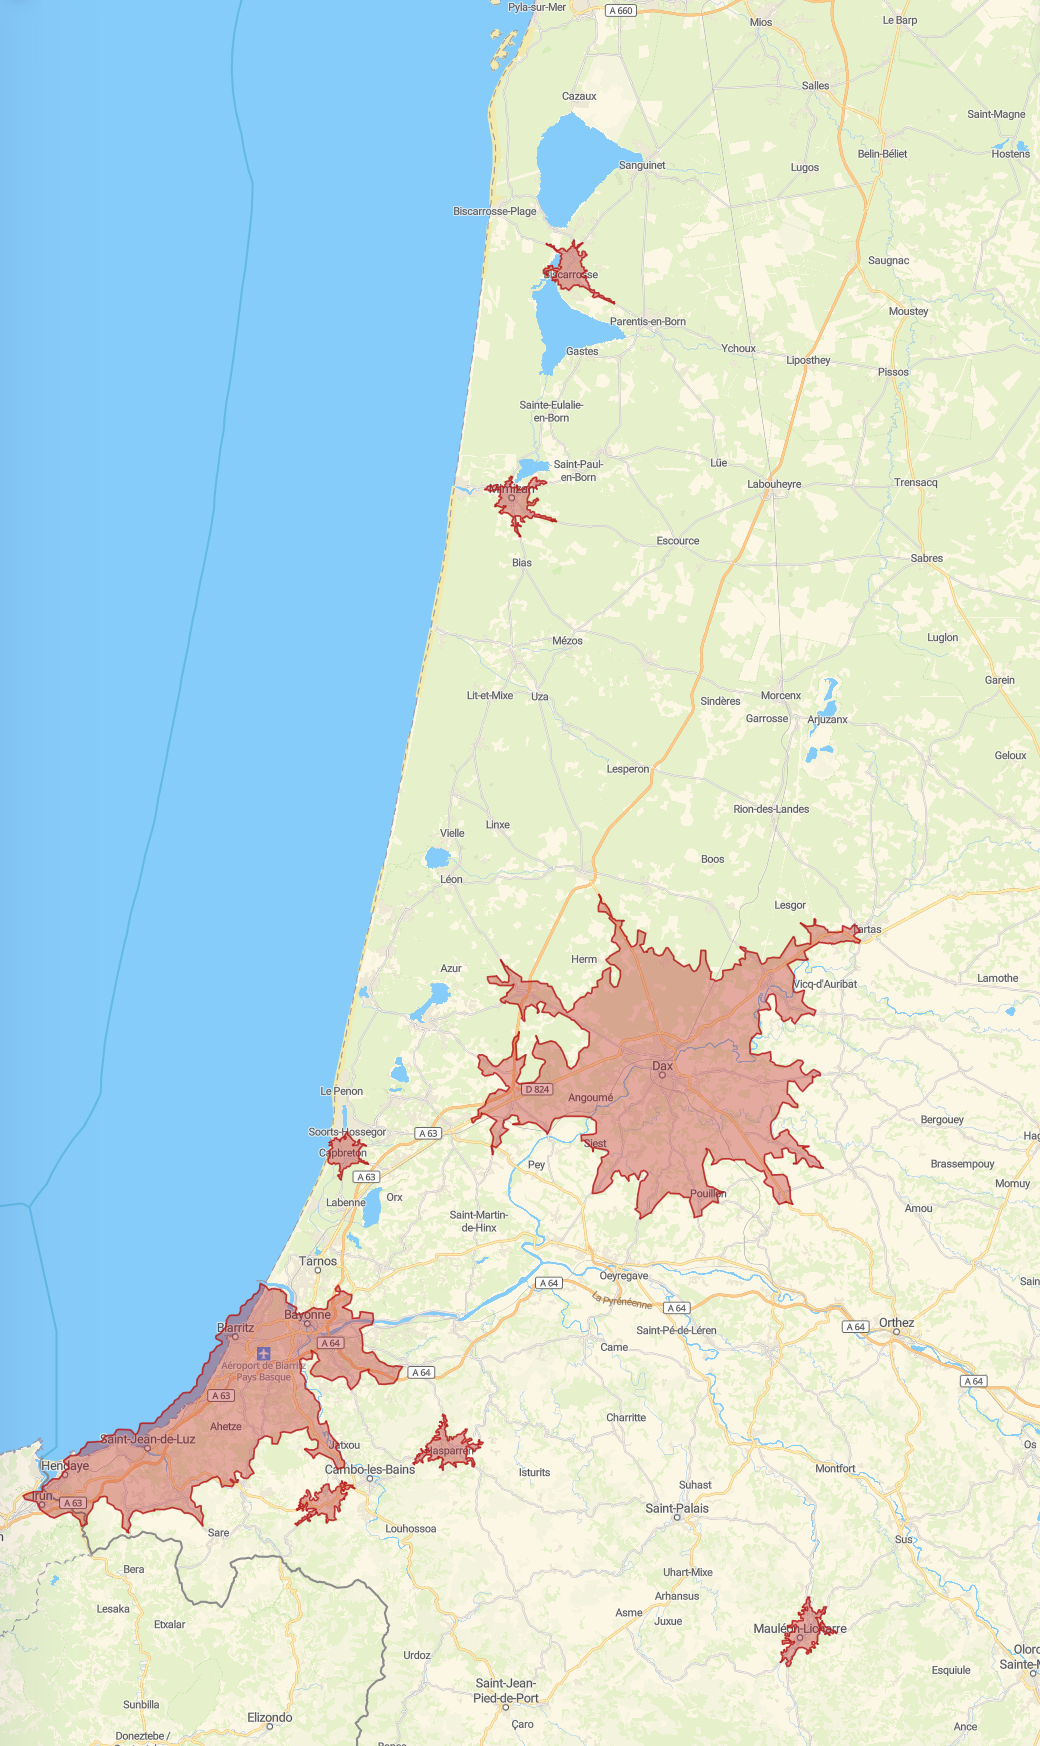
\includegraphics[scale=0.2]{zone_chalandise_aditu.png}
%     \figurename
%     \caption{Visualisation de la zone de chalandise d'ADITU, regroupée autour de ses datacenters à Bidart et à Dax}
%     \label{fig:zone_chalandise}
% \end{figure}

% \section{Cahier des charge Ticketing}

% % \begin{figure}[H]
% %     \centering
% %     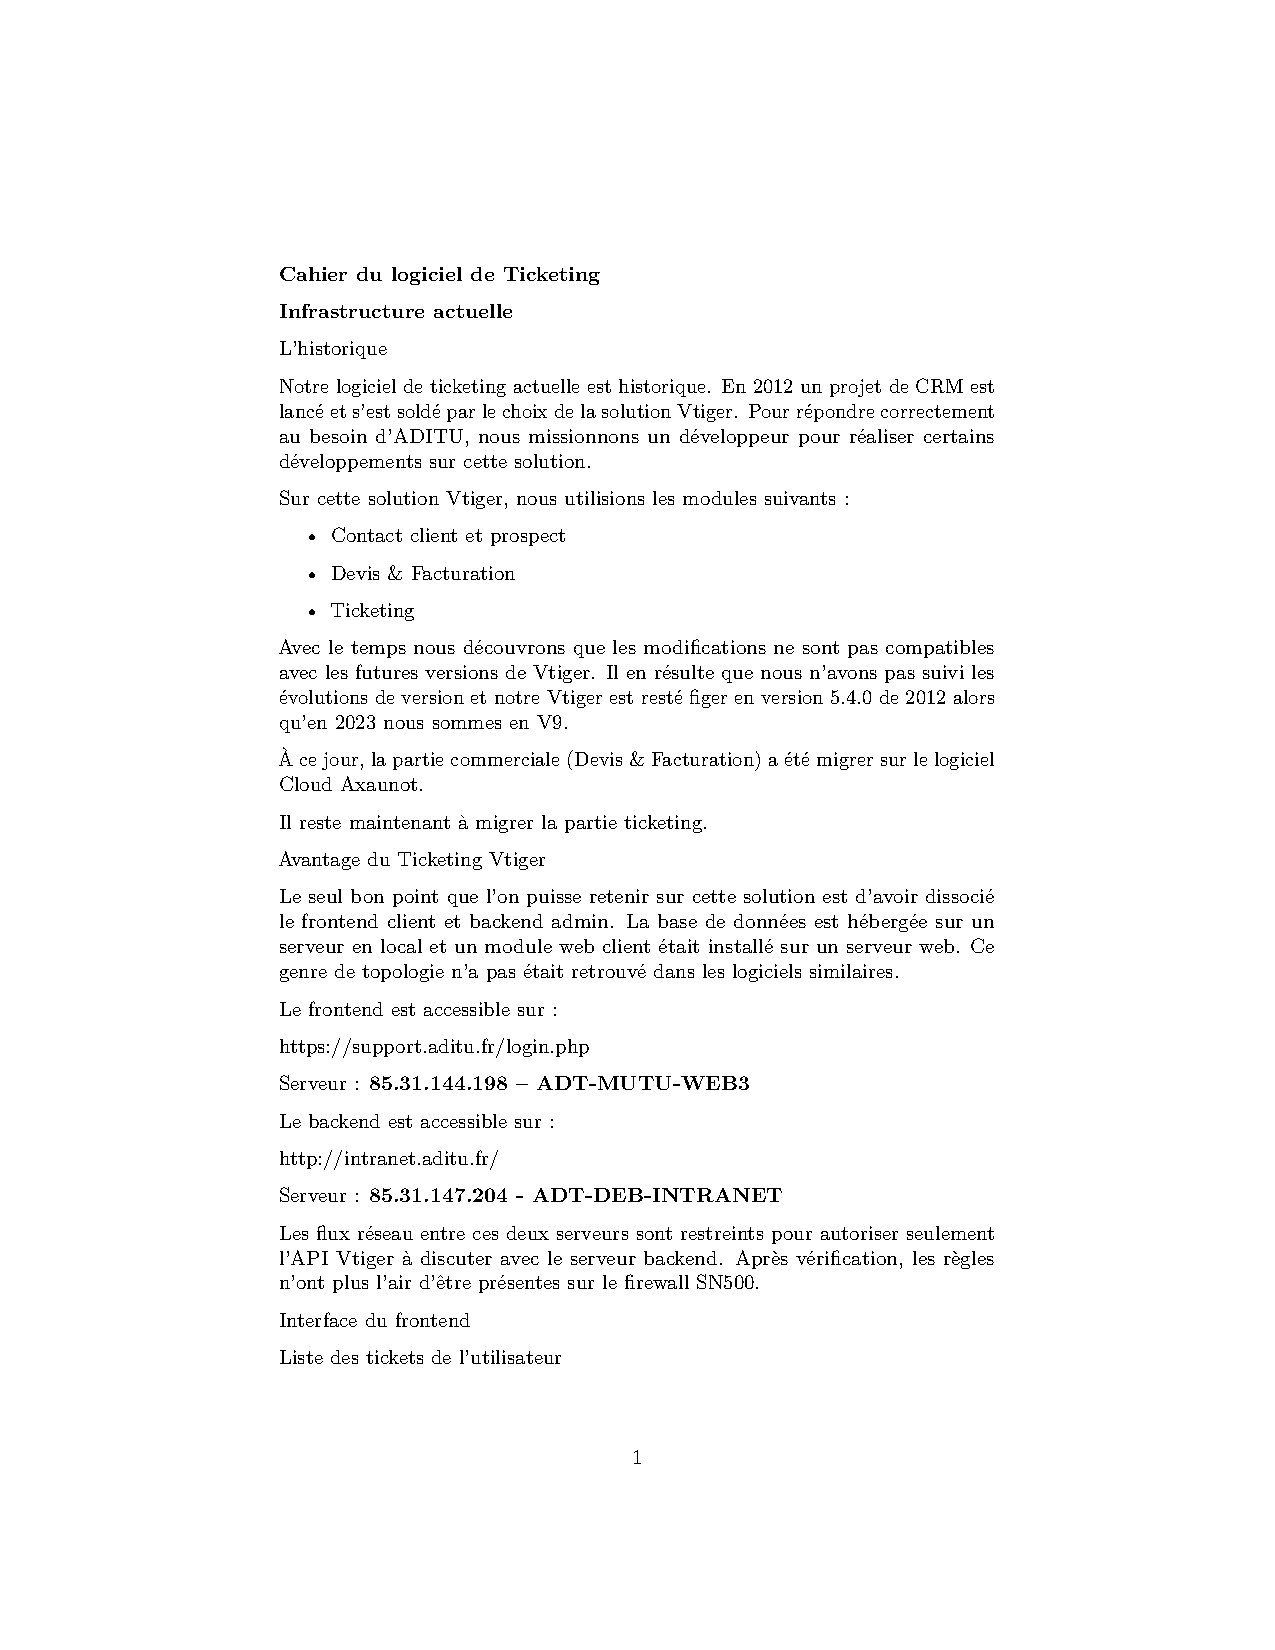
\includegraphics[width=\textwidth - \textwidth / 20]{CDC-Ticketing.pdf}
% %     \figurename
% %     \caption{Fiche de poste de notre alternance}
% %     \label{fig:poste}
% % \end{figure}

% \textbf{Cahier du logiciel de Ticketing}

% \textbf{Infrastructure actuelle}

% L'historique

% Notre logiciel de ticketing actuelle est historique. En 2012 un projet
% de CRM est lancé et s'est soldé par le choix de la solution Vtiger. Pour
% répondre correctement au besoin d'ADITU, nous missionnons un développeur
% pour réaliser certains développements sur cette solution.

% Sur cette solution Vtiger, nous utilisions les modules suivants~:

% \begin{itemize}
% \item
%   Contact client et prospect
% \item
%   Devis \& Facturation
% \item
%   Ticketing
% \end{itemize}

% Avec le temps nous découvrons que les modifications ne sont pas
% compatibles avec les futures versions de Vtiger. Il en résulte que nous
% n'avons pas suivi les évolutions de version et notre Vtiger est resté
% figer en version 5.4.0 de 2012 alors qu'en 2023 nous sommes en V9.

% À ce jour, la partie commerciale (Devis \& Facturation) a été migrer sur
% le logiciel Cloud Axaunot.

% Il reste maintenant à migrer la partie ticketing.

% Avantage du Ticketing Vtiger

% Le seul bon point que l'on puisse retenir sur cette solution est d'avoir
% dissocié le frontend client et backend admin. La base de données est
% hébergée sur un serveur en local et un module web client était installé
% sur un serveur web. Ce genre de topologie n'a pas était retrouvé dans
% les logiciels similaires.

% Le frontend est accessible sur~:

% \url{https://support.aditu.fr/login.php}

% Serveur~: \textbf{85.31.144.198 -- ADT-MUTU-WEB3}

% Le backend est accessible sur~:

% \url{http://intranet.aditu.fr/}

% Serveur~: \textbf{85.31.147.204 - ADT-DEB-INTRANET}

% Les flux réseau entre ces deux serveurs sont restreints pour autoriser
% seulement l'API Vtiger à discuter avec le serveur backend. Après
% vérification, les règles n'ont plus l'air d'être présentes sur le
% firewall SN500.

% Interface du frontend

% Liste des tickets de l'utilisateur

% 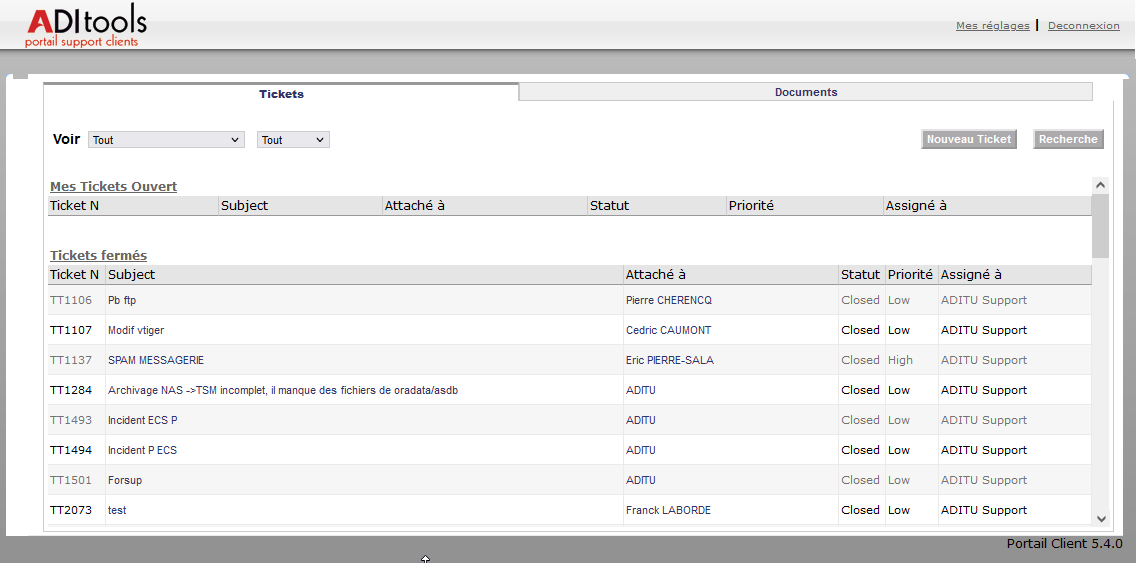
\includegraphics[width=6.3in,height=3.12222in]{image1.png}

% Création de tickets

% 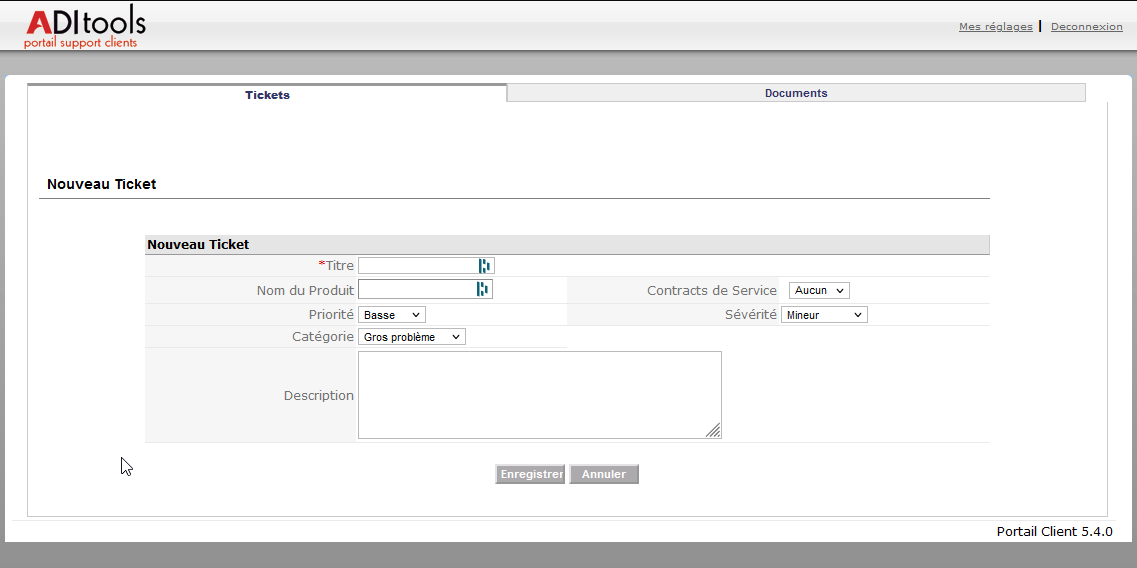
\includegraphics[width=6.3in,height=3.14722in]{image2.png}

% On peut constater que l'interface est plutôt minimaliste et
% vieillissante. Il manque certaines fonctions qui seront abordées plus
% bas.

% \textbf{Nouveau logiciel souhaité}

% Nous souhaitons migrer vers un nouveau logiciel de ticketing qui puisse
% intégrer les fonctionnalités ci-dessous~:

% Création d'incidents

% \begin{quote}
% La gestion des incidents permet de suivre et de résoudre les incidents
% signalés par les utilisateurs.
% \end{quote}

% Création de demandes de changement

% \begin{quote}
% Gestion des changements permet de planifier, suivre et gérer les
% modifications demandées par les utilisateurs.

% Exemple~: modification de ports sur le firewall, augmenter une boite aux
% lettres, etc.
% \end{quote}

% Création de tickets automatiquement

% \begin{quote}
% Cette fonctionnalité permet de planifier des interventions récurrentes
% sans les oublier. Exemple~: test de restauration
% \end{quote}

% Gestion des ressources

% \begin{quote}
% Pouvoir lié du matériel ou logiciel a un client et faire un suivi des
% modifications sur ce cette ressource.

% Exemple~: avoir le suivi des modifications comme celui qui est présent
% sur la page client du wiki.

% Intégrer du matériel lié à un fournisseur et gérer sa garantie. Exemple
% NAS ANANDA.

% Gérer les renouvellements~: des certificats

% Gérer les renouvellements~: des noms de domaines
% \end{quote}

% Inventaires

% \begin{quote}
% Lister l'ensemble des machines (connecteur OCS)
% \end{quote}

% Tableaux de bord et rapports

% Avoirs des stats et indicateurs sur ce qui nous prend le plus de temps
% dans le support.

% Ergonomique

% \begin{quote}
% Il faut que le logiciel soit intuitif et ergonomique. Que l'utilisateur
% ne soit pas rebuté par la complexité d'ouverture d'un ticket.
% \end{quote}

% Ouverture de ticket via email

% Fermeture de ticket automatique après un délai de non-réponse

% Personnalisation graphique

% \begin{quote}
% Nous souhaitons que l'application puisse se personnaliser aux couleurs
% de la société et d'y insérer le logo.
% \end{quote}

% Récupération des données ticketing vtiger

% \begin{quote}
% Seulement si cette récupération est facile. Ne pas perdre du temps sur
% cette récupération.
% \end{quote}

% Fonctions annexes

% Gestion des baies racks du datacenter


\end{document}
